
\documentclass[a4paper,11pt]{article}%,twocolumn
%% packages

\usepackage{blindtext} % needed for creating dummy text passages
%\usepackage{ngerman} % needed for German default language
\usepackage{amsmath} % needed for command eqref
\usepackage{amssymb} % needed for math fonts
\usepackage[colorlinks=true,breaklinks]{hyperref} % needed for creating hyperlinks in the document, the option colorlinks=true gets rid of the awful boxes, breaklinks breaks lonkg links (list of figures), and ngerman sets everything for german as default hyperlinks language
\usepackage[hyphenbreaks]{breakurl} % ben�tigt f�r das Brechen von URLs in Literaturreferenzen, hyphenbreaks auch bei links, die �ber eine Seite gehen (mit hyphenation).
\usepackage{xcolor}
\definecolor{c1}{rgb}{0,0,1} % blue
\definecolor{c2}{rgb}{0,0.3,0.9} % light blue
\definecolor{c3}{rgb}{0.3,0,0.9} % red blue
\hypersetup{
    linkcolor={c1}, % internal links
    citecolor={c2}, % citations
    urlcolor={c3} % external links/urls
}
%\usepackage{cite} % needed for cite
\usepackage[square,authoryear]{natbib} % needed for cite and abbrvnat bibliography style
\usepackage[nottoc]{tocbibind} % needed for displaying bibliography and other in the table of contents
\usepackage{graphicx} % needed for \includegraphics 
\usepackage{longtable} % needed for long tables over pages
\usepackage{bigstrut} % needed for the command \bigstrut
\usepackage{enumerate} % needed for some options in enumerate
%\usepackage{todonotes} % needed for todos
\usepackage{makeidx} % needed for creating an index
\makeindex
\usepackage{gensymb}
\usepackage{url}
\usepackage{psfrag}
\usepackage{multirow}
\usepackage{subfigure}
%% page settings

\usepackage[top=20mm, bottom=20mm,left=15mm,right=15mm]{geometry} % needed for page border settings
\parindent=0mm % for space of first line of new text block
\sloppy % for writing with hyphenless justification (tries to)
\hyphenation{} % use hyphenation of tolerance parametershttp://www.jr-x.de/publikationen/latex/tipps/zeilenumbruch.html
\hyphenpenalty=10000
\exhyphenpenalty=10000
\usepackage{fancyhdr} % needed for head and foot options
%% my macros

%% Text fomats
\newcommand{\tbi}[1]{\textbf{\textit{#1}}}

%% Math fonts
\newcommand{\bbA}{\mathbb{A}}
\newcommand{\bbB}{\mathbb{B}}
\newcommand{\bbC}{\mathbb{C}}
\newcommand{\bbD}{\mathbb{D}}
\newcommand{\bbE}{\mathbb{E}}
\newcommand{\bbF}{\mathbb{F}}
\newcommand{\bbG}{\mathbb{G}}
\newcommand{\bbH}{\mathbb{H}}
\newcommand{\bbI}{\mathbb{I}}
\newcommand{\bbJ}{\mathbb{J}}
\newcommand{\bbK}{\mathbb{K}}
\newcommand{\bbL}{\mathbb{L}}
\newcommand{\bbM}{\mathbb{M}}
\newcommand{\bbN}{\mathbb{N}}
\newcommand{\bbO}{\mathbb{O}}
\newcommand{\bbP}{\mathbb{P}}
\newcommand{\bbQ}{\mathbb{Q}}
\newcommand{\bbR}{\mathbb{R}}
\newcommand{\bbS}{\mathbb{S}}
\newcommand{\bbT}{\mathbb{T}}
\newcommand{\bbU}{\mathbb{U}}
\newcommand{\bbV}{\mathbb{V}}
\newcommand{\bbW}{\mathbb{W}}
\newcommand{\bbX}{\mathbb{X}}
\newcommand{\bbY}{\mathbb{Y}}
\newcommand{\bbZ}{\mathbb{Z}}
\usepackage[ framed, numbered]{matlab-prettifier}%framed,%
\usepackage{listings}
\usepackage{physics}
\usepackage{pdfpages}
\usepackage[toc,page]{appendix}
\usepackage{float}
\usepackage{hyperref}

% for code
\usepackage{listings}
\usepackage{color}
% Define colors
\definecolor{codegreen}{rgb}{0,0.6,0}
\definecolor{codegray}{rgb}{0.5,0.5,0.5}
\definecolor{codepurple}{rgb}{0.58,0,0.82}
\definecolor{backcolour}{rgb}{0.95,0.95,0.92}
% Setup the listings package
\lstset{
    backgroundcolor=\color{backcolour},   
    commentstyle=\color{codegreen},
    keywordstyle=\color{magenta},
    numberstyle=\tiny\color{codegray},
    stringstyle=\color{codepurple},
    basicstyle=\footnotesize,
    breakatwhitespace=false,         
    breaklines=true,                 
    captionpos=b,                    
    keepspaces=true,                                
    showspaces=false,                
    showstringspaces=false,
    showtabs=false,                  
    tabsize=2
}

\newenvironment{qanda}{\setlength{\parindent}{0pt}}{\bigskip}
\newcommand{\Q}{\bigskip\bfseries Q: }
\newcommand{\A}{\par\textbf{Answer: } \normalfont}

\begin{document}
\begin{titlepage}
\center % Center everything on the page

%-------------------------------------------------------------------------------------
%	HEADING SECTIONS
%------------------------------------------------------------------------------------
\textbf{\large Department of Electrical and Computer Engineering}\\[0.5cm]
\textbf{\Large University of Colorado at Boulder}\\[1cm]
\textbf{\large ECEN5623 - Real Time Embedded Systems }\\[2cm]

\includegraphics[width=0.3\textwidth]{figures/cu}\\[2cm]

	
%-------------------------------------------------------------------------------------
%	TITLE SECTION
%------------------------------------------------------------------------------------
\textbf{\Huge Exercise 5 }\\[0.2cm]



%----------------------------------------------------------------------------------------
%	MEMBERS SECTION
%----------------------------------------------------------------------------------------


\vfill

\textbf{\large Submitted by}\\[0.5cm]

{\large Parth | Jithedra}\\[0.5cm]	

%----------------------------------------------------------------------------------------
%	DATE SECTION
%----------------------------------------------------------------------------------------

\textbf{\large Submitted on}
\textbf{\Large \today} % Date, change the \today to a set date if you want to be precise

%----------------------------------------------------------------------------------------

\vfill % Fill the rest of the page with whitespace

\end{titlepage}


\pagebreak

\tableofcontents
\listoffigures
\listoftables
\vfill
\begin{center}
    \textbf{\textit{*PDF is clickable}}
\end{center}

\pagebreak

\section{Team Members Name}

\textbf{Parth Thakkar }\\[0.2cm]
\textbf{Tirth Patel }\\[0.2cm]

\pagebreak

\section{Introduction}
In the embedded systems and computer vision, the Hawkeye project shows real-time face tracking and laser pointing. By leveraging the Linux POSIX API and embedded Linux, Hawkeye aims to create a sophisticated system that can detect, track, and engage with human faces in real-time, all while adhering to strict deadlines and ensuring deterministic performance.
\subsection{Objectives}
The primary objective of the Hawkeye project is to develop a efficient face tracking and laser pointing system that can operate within strict real-time constraints. The system should be capable of capturing frames at a minimum rate of 20 frames per second (FPS), allowing for a maximum computation time of 50ms for image processing, face detection, and coordinate extraction.
\subsection{Use Case}
\begin{itemize}
    \item The gaming and entertainment industry can also benefit greatly from the Hawkeye system. By integrating face tracking and laser pointing into gaming experiences, developers can create immersive and interactive gameplay mechanics that respond to players' facial expressions and movements.
    \item In the domain of security and surveillance, Hawkeye can be utilized to monitor and track individuals in restricted areas or high-security facilities. By accurately detecting and tracking faces, the system can help identify potential threats or unauthorized personnel, enhancing overall security measures. While the project currently focuses on laser pointing for demonstration purposes, future iterations could explore the integration of more advanced security features.
    \item Interactive advertising is another area where the Hawkeye system can make a significant impact. By incorporating face tracking and laser pointing into digital signage and billboards, advertisers can create targeted and personalized experiences for consumers. The system can detect and track the faces of passersby, using the laser pointer to highlight specific products or promotions based on their gaze or attention.
    \item The Hawkeye project has applications in the field of augmented reality (AR). By leveraging face tracking and laser pointing, the system can enable users to interact with virtual objects and navigate AR interfaces using natural and intuitive facial movements. This can create immersive AR experiences in various domains, including education, training, entertainment, and industrial applications.
\end{itemize}

\begin{figure}[H]
    \centering
    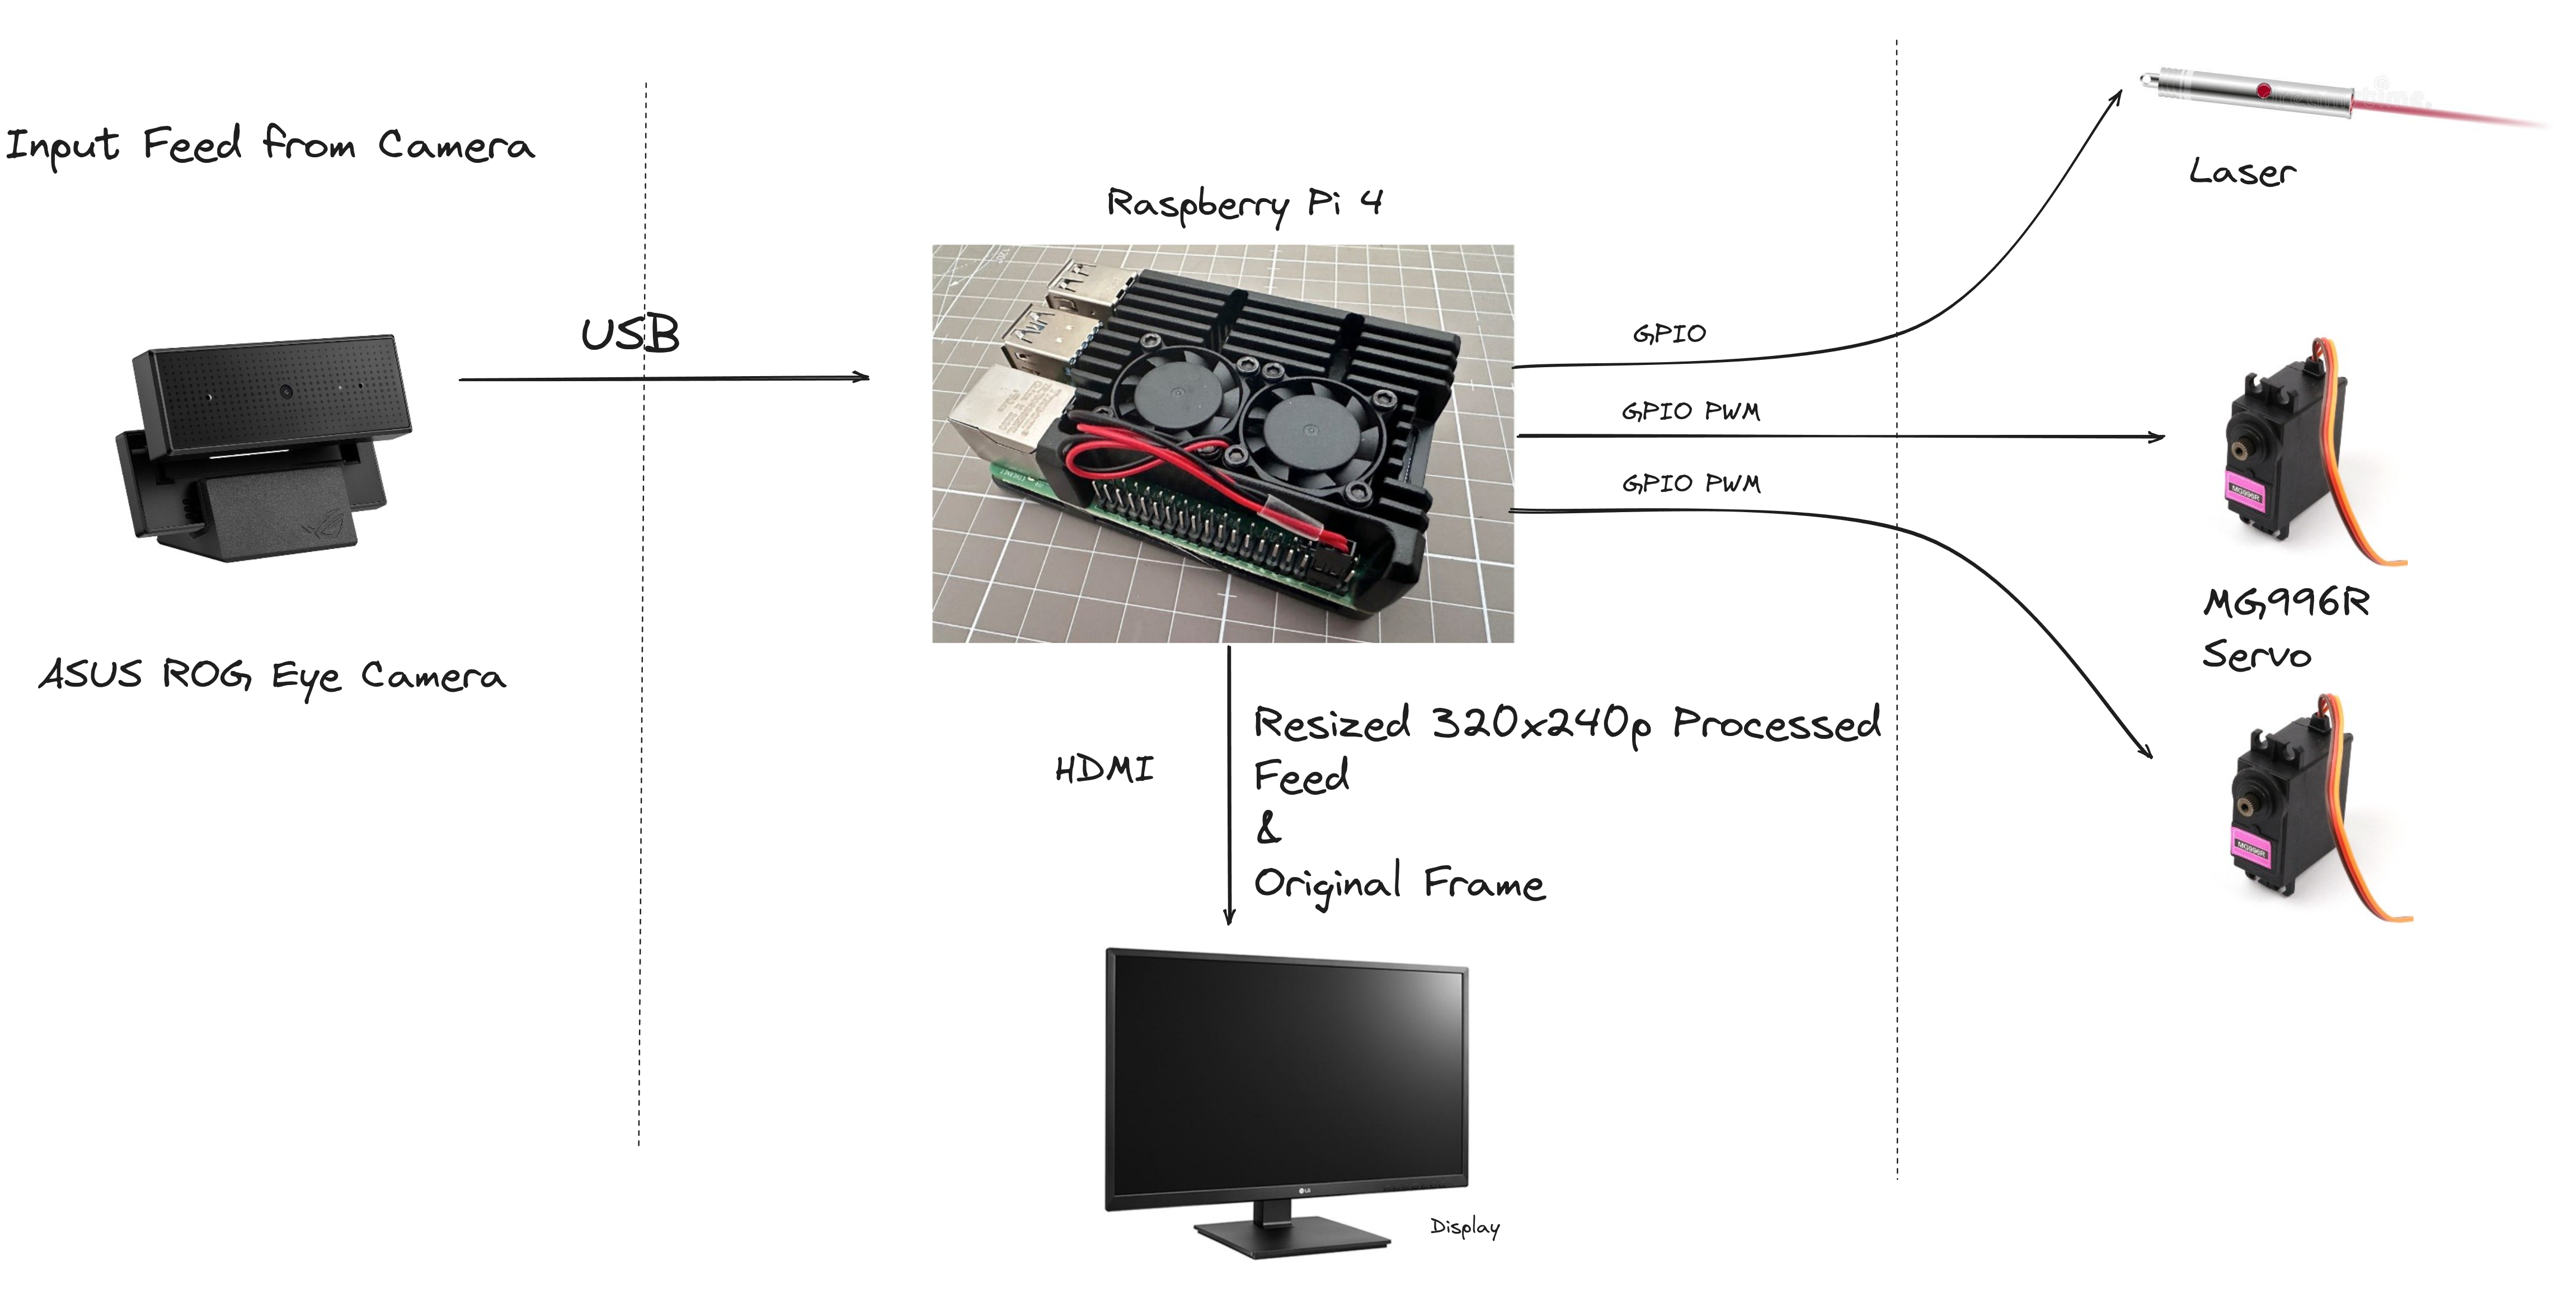
\includegraphics[scale=0.1]{figures/hw_overview.png}
    \caption{Hardware Components}
\end{figure}

\begin{figure}[H]
    \centering
    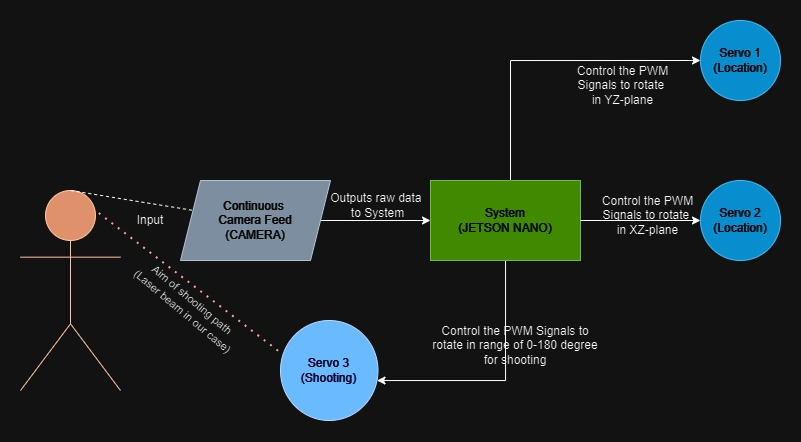
\includegraphics[scale=0.6]{figures/hw_overview.jpeg}
    \caption{Hardware Components}
\end{figure}

\section{Functional Requirements}
The Hawkeye project is a system that combines face tracking, servo control, and laser pointing capabilities. To ensure the system meets its intended objectives and performs reliably in real-time, a set of well-defined functional requirements is essential. This section outlines the key functional requirements for the Hawkeye project, covering aspects such as frame capture and processing, servo control, inter-process communication (IPC), and predefined distance constraint.
\subsection{Sequencer}
Sequencer would be running at 20 Hz that is every 50 ms to release all the services Sequence would run on core 1 where service 2 and three are running and core 0 would be utilized for face detection service.

\subsection{Frame Capture and Processing}
One of the fundamental requirements of the Hawkeye system is the ability to capture and process frames in real-time. The following functional requirements pertain to frame capture and processing:
\begin{itemize}
    \item \textbf{FR1.1}: The system will capture frames at a minimum rate of 20 frames per second (FPS) to ensure smooth and responsive face tracking.
    \item \textbf{FR1.2}: The maximum computation time for image processing, face detection, and coordinate extraction will not exceed 50 milliseconds per frame (deadline), allowing for real-time performance.
    \item \textbf{FR1.3}: The face detection algorithm will utilize a lightweight Haar Cascade classifier optimized for embedded systems (lbp haar cascade) to achieve efficient face detection.
    \item \textbf{FR1.4}: The system will process gray-scale images with a reduced dimension of 320x240 pixels to optimize computational efficiency while maintaining sufficient resolution for face detection up to a distance of 4 meters, which is within the predefined distance for shooting of 1 meters.
    \item \textbf{FR1.5}: The face detection service will achieve a minimum detection accuracy of 80\%.
\end{itemize}
\subsection{Servo Control}
The Hawkeye system relies on servo control to accurately point the laser at detected faces. The following functional requirements specify the servo control capabilities:
\begin{itemize}
    \item \textbf{FR2.1}: The system will utilize two servos: one for controlling the pan (rotation in the XZ plane) and another for controlling the tilt (rotation in the YZ plane) of the laser pointer.
    \item \textbf{FR2.2}: The servos will be actuated using hardware PWM (Pulse Width Modulation) to ensure precise and deterministic control.
    \item \textbf{FR2.3}: A hardware timer will be employed to generate the required PWM output at the servo signal pin, ensuring accurate timing and minimizing jitter for the 50Hz PWM signal .
    \item \textbf{FR2.4}: The system shall optimize the electrical control time for sending signals to the servos to meet the project's deadline, while acknowledging the mechanical movement time of the servos is beyond direct control. from the data-sheet we can see tha physical movement of the servo is around this this degree per sec. which is beyond our control.
    \item \textbf{FR2.5} First I had used software PWM to generate the PWM signal to control pins which was not efficiat as it was taking around 20 ms of time for the response which was not feasible so I moved to raspberry pi for Hardware based PWM.
\end{itemize}
\subsection{Services and Inter-Process Communication (IPC)}
The Hawkeye system consists of multiple services that need to communicate and coordinate with each other. The following functional requirements outline the services and their IPC mechanisms:
\begin{itemize}
    \item \textbf{FR3.1}: The system shall comprise three main services:
          \begin{enumerate}
              \item Frame capture, face recognition, and face processing service
              \item Servo actuation service: calculates pan and tilt for the servo.
              \item Shooting service, responsible for turning on the laser when a face is detected and the servo has been actuated to the face coordinates by servo Actuation service
          \end{enumerate}
    \item \textbf{FR3.2}: IPC message queues is utilized to transfer face detection points from the face detection service to the servo actuation service, to signal servo service to calculate pan and tilt
    \item \textbf{FR3.3}: Semaphores is be employed to synchronize the servo actuation and shooting services, guaranteeing sequential execution and preventing any race conditions or conflicts.
\end{itemize}
\subsection{Predefined Distance Constraint}
To simplify the project and meet the tight development timeline, the Hawkeye system operates under a predefined distance constraint (1 meter). The following functional requirements specify this constraint:
\begin{itemize}
    \item \textbf{FR4.1}: The system shall assume a predefined distance of 1 meter between the camera and the target face for face detection and mathematical calculations.
    \item \textbf{FR4.2}: By adopting this predefined distance constraint, the system can eliminate the need for additional sensors such as LDR, ultrasonic, or LiDAR, reducing the complexity of the project while still providing reliable face tracking functionality.
\end{itemize}


\section{Real-Time Requirements}
The Hawkeye project is a real-time embedded system that demands strict adherence to timing constraints and deterministic behavior. To ensure the system meets its objectives, a set of well-defined real-time requirements has been made. This section outlines the key real-time requirements for the Hawkeye project, including response time, deadlines, execution times, and task allocation.
\subsection{Response Time and Deadline}
One of the critical aspects of the Hawkeye system is its ability to respond quickly and accurately to detected faces. The following real-time requirements pertain to response time and deadline:
\begin{itemize}
    \item \textbf{RTR1.1}: The overall system response time, from face detection to laser pointing, shall not exceed 152 milliseconds. This requirement is derived from research studies on human perception and reaction times. The total deadline/response time is limited to less than 164ms based on a paper that surveyed the reaction time of sprinters' body parts when a gun is fired. Considering that our laser targets the face, we accounted for the reaction time of the shoulder, which is stated as 164 ± 12ms. To ensure a responsive system, we aimed for a response time less than 164ms and decided on a total deadline of 152ms.


          \begin{figure}[H]
              \centering
              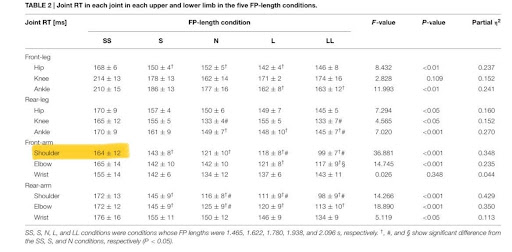
\includegraphics[scale=0.8]{figures/face_detection_paper.png}
              \caption{Response Time Research Paper}
          \end{figure}

          Paper Source: “Timing of Gun Fire Influences Sprinters’ Multiple Joint Reaction Times of Whole Body” – Frontiers of Psychology


    \item \textbf{RTR1.2}: The system shall have a fixed deadline of 152 milliseconds for completing all tasks, including frame capture, face detection, servo actuation, and laser pointing. Meeting this deadline ensures that the system provides a smooth and responsive user experience.
    \item \textbf{RTR1.3}  The deadline for the Face Detection service is determined based on a research paper that compares the processing time for face recognition between CPU and GPU implementations.\\
          According to the paper, face recognition on a CPU is processed in 52ms at 24 frames per second (fps), while on a GPU, it is processed in 47ms at 24 fps.\\
          Considering the CPU processing time as a reference, we set the deadline for the Face Detection service to 50ms.
          This deadline ensures that the Face Detection service can process frames at a rate of approximately 20 fps (1000ms / 50ms = 20 fps), which meets the real-time requirements of the system.

          \begin{figure}[H]
              \centering
              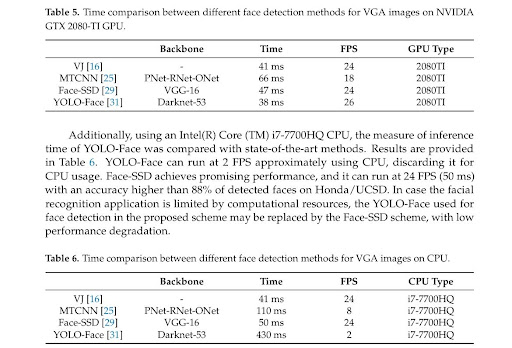
\includegraphics[scale=0.6]{figures/face_detection_service_papeere.png}
              \caption{Face Detection Research Paper}
          \end{figure}
          Paper Source: “Efficient Face Recognition System for Operating in Unconstrained Environments” – Journal of Imaging, MDPI

\end{itemize}

\subsection{Service Deadlines and Execution Times}

\begin{figure}[H]
    \centering
    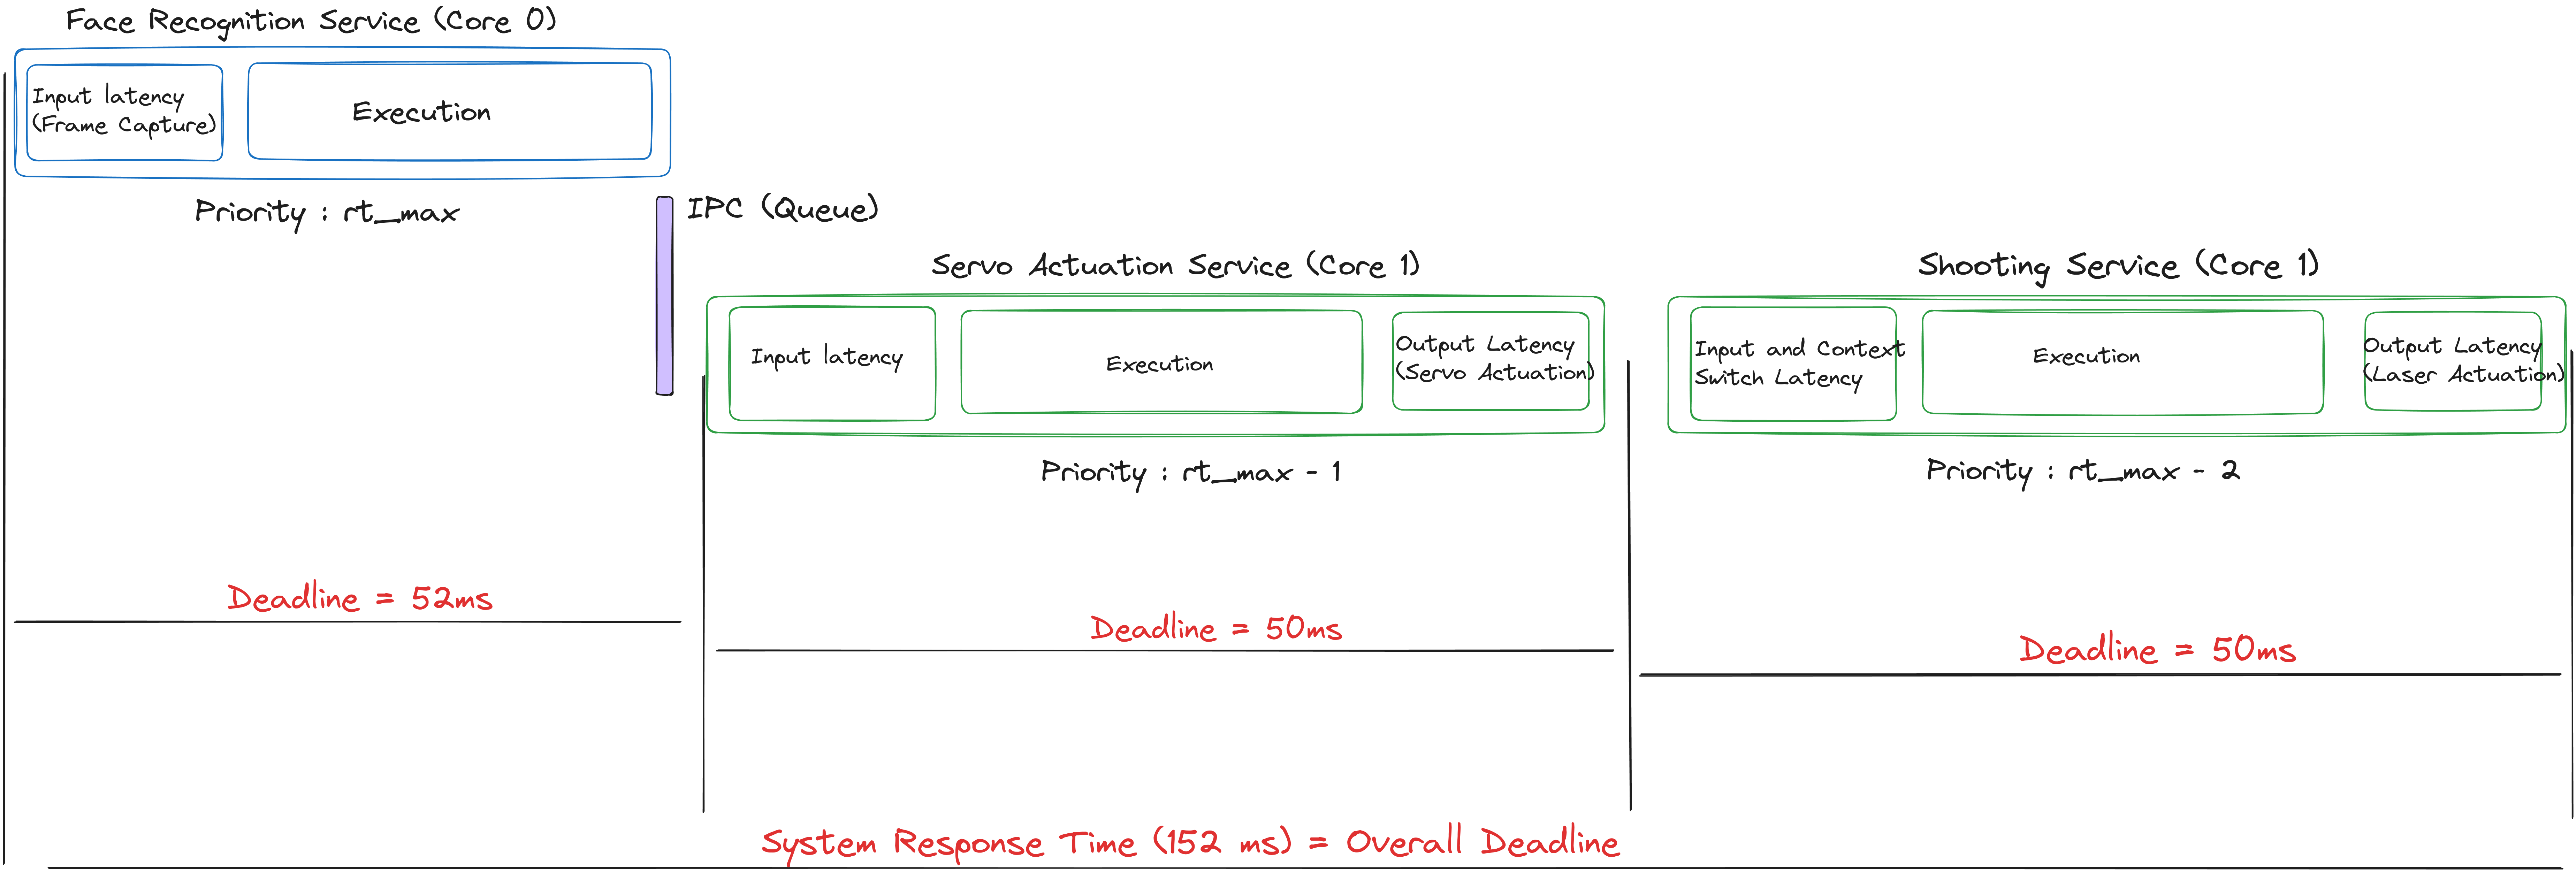
\includegraphics[scale=0.06]{figures/response_time.png}
    \caption{CPU Utilization}
\end{figure}


To meet the overall system deadline of 152 milliseconds, each individual service within the Hawkeye system must adhere to specific deadlines and execution times. The following real-time requirements define the timing constraints for each service:
\begin{itemize}
    \item \textbf{RTR2.1}: The frame capture, face detection, and face processing service shall have a deadline (D1) of 52 milliseconds and a period (T1) of 50 milliseconds. This requirement ensures that the system can process frames at a rate of 20 FPS, providing smooth and responsive face tracking.
    \item \textbf{RTR2.2}: The execution time (C1) of the frame capture, face detection, and face processing service should be less than 50 milliseconds.
    \item \textbf{RTR2.3}: The servo actuation service shall have a deadline (D2) of 50 milliseconds and a period (T2) of 50 milliseconds. We have given this deadline to divide the overall response time to 152 ms.
    \item \textbf{RTR2.4}: The execution time (C2) of the servo actuation service shall be within 3-4 milliseconds. This requirement ensures that the servo actuation service can complete its tasks efficiently and leave enough time for other services to execute within the overall system deadline.
    \item \textbf{RTR2.5}: The servo shooting service shall have a deadline (D3) of 50 milliseconds and a period (T3) of 50 milliseconds. This requirement allows the servo shooting service to coordinate with the servo actuation service and trigger the laser pointer at the appropriate time.
    \item \textbf{RTR2.6}: The execution time (C3) of the servo shooting service shall be within 3-4 milliseconds. This requirement guarantees that the servo shooting service can perform its tasks quickly and efficiently, minimizing any additional latency in the system.
\end{itemize}
The deadlines and execution times for each service are carefully chosen based on the overall system deadline of 152 milliseconds and the interdependencies between the services. These requirements ensure that the system can perform all necessary tasks within the allocated time budget, providing a responsive and real-time user experience.

\begin{table}[H]
    \centering
    \begin{tabular}{|l|c|c|c|c|c|}
    \hline
    Task & Proposed ($C_i$) & Deadline ($D_i$) & Period ($T_i$) & Obtained $C_{avg}$ & Obtained $C_{wcet}$  \\
    \hline
    Task 1 (T1) & 35ms & 52ms & 50ms & 25ms & 26.75ms\\
    Task 2 (T2) & 4ms & 50ms & 50ms & 0.2ms & 0.24ms\\
    Task 3 (T3) & 3ms & 50ms & 50ms & 0.1ms & 0.2ms\\
    \hline
    \end{tabular}
\caption{Task Parameters}
\end{table}
Table summarizes the deadlines, periods, and execution times for each service in the system. These values are derived based on the real-time requirements and the system's overall timing constraints.
\subsection{Task Allocation and Scheduling}
To ensure the system meets its real-time requirements and achieves optimal performance, careful task allocation and scheduling are necessary. The following real-time requirements address task allocation and scheduling:\\
The sequencer is running at 50 Hz with the highest priority, giving a semaphore to each service every 50 ms. The frame capture has the highest priority, while servo actuation has lower priority, and the servo shoot service has even lower priority.

\begin{itemize}
    \item \textbf{RTR3.1}: The frame capture, face detection, and face processing tasks shall be allocated to Core 0 of the processor. This requirement ensures that these computationally intensive tasks have dedicated resources and can execute without interference from other tasks.
    \item \textbf{RTR3.2}: The servo actuation and servo shooting tasks shall be allocated to Core 1 of the processor.
    \item \textbf{RTR3.3}: The frame capture, face detection, and face processing tasks shall have the highest priority among all tasks.
    \item \textbf{RTR3.4}: The servo actuation task shall have a lower priority than the frame capture, face detection, and face processing tasks, but higher than the servo shooting task. This requirement ensures that the servo actuation task executes after the face detection tasks and provides the necessary data for the servo shooting task.
    \item \textbf{RTR3.5}: The servo shooting task shall have the lowest priority among all tasks. As it depends on servo actuation service to be executed first
\end{itemize}
Figure illustrates the task allocation and scheduling in the Hawkeye system. The frame capture, face detection, and face processing tasks are allocated to Core 0, while the servo actuation and servo shooting tasks are allocated to Core 1. The priorities of the tasks are assigned based on their criticality and dependencies.
\begin{figure}[H]
    \centering
    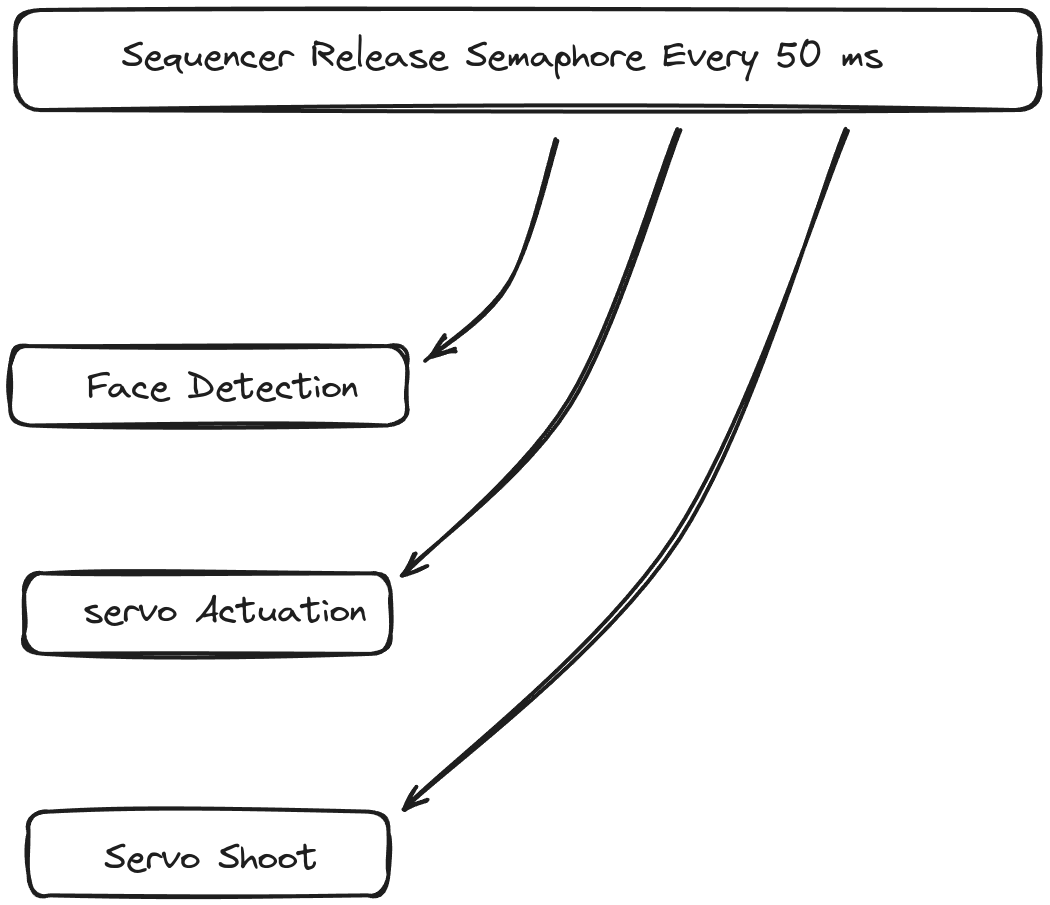
\includegraphics[scale=0.25]{figures/task_allocation.png}
    \caption{Task Allocation via sequencer}
\end{figure}

By allocating tasks to specific processor cores and assigning appropriate priorities, the system can ensure that each task receives the necessary resources and execution time to meet its real-time requirements. This allocation and scheduling scheme helps to optimize the system's performance, minimize interference between tasks, and guarantee the timely execution of critical tasks.

\subsection{System Feasibility and Analysis}
To validate the feasibility of the Hawkeye system and ensure that it meets its real-time requirements, a thorough analysis of the system's timing properties is essential. The following real-time requirements pertain to system feasibility and analysis:
\begin{itemize}
    \item \textbf{RTR4.1}: We have done cheddar analysis for the task with Rate monotonic schedular, According to cheddar the system is feasible
          \begin{figure}[H]
              \centering
              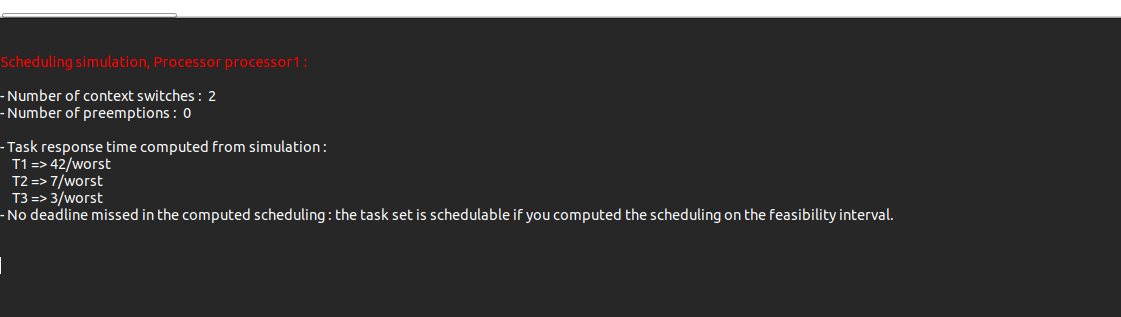
\includegraphics[scale=0.4]{figures/c.png}
              \caption{Scheduling output}
          \end{figure}
          \begin{figure}[H]
              \centering
              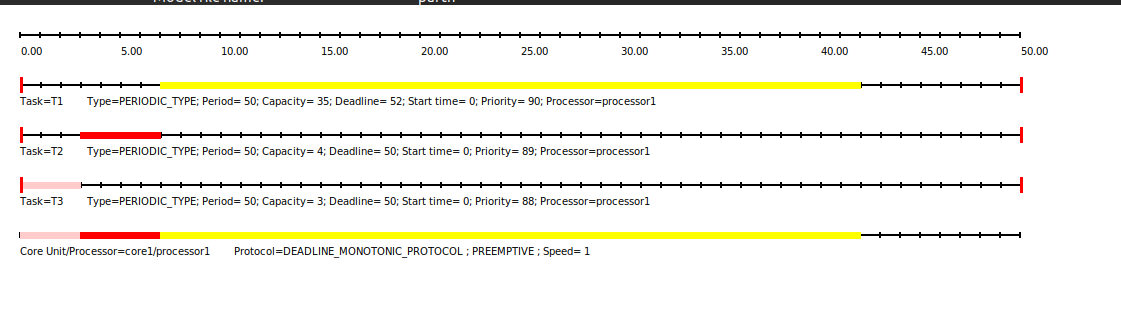
\includegraphics[scale=0.4]{figures/c1.png}
              \caption{Cheddar Scheduling}
          \end{figure}
          \begin{figure}[H]
              \centering
              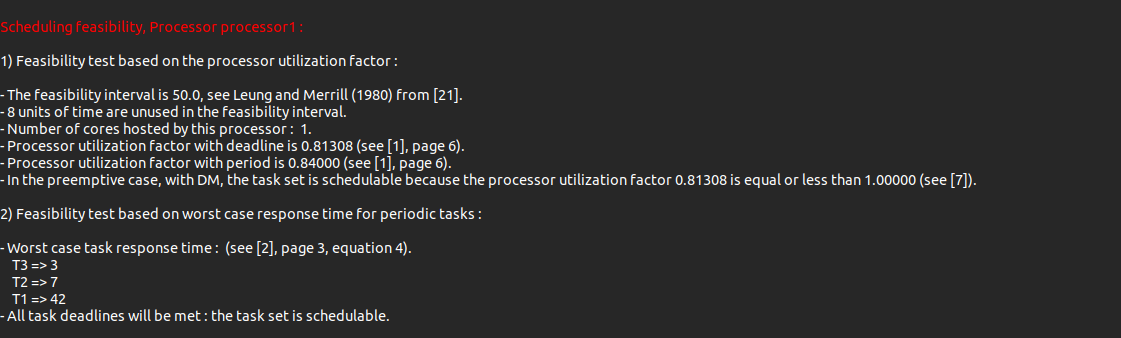
\includegraphics[scale=0.4]{figures/c3.png}
              \caption{Feasiblility Test cheddar}
          \end{figure}
    \item \textbf{RTR4.2}: We have done Scheduling Point analysis and Completion time feasibility with help of Excercise 2 code. also according to necessary and sufficient test analysis we can say that the system is feasible.
          \begin{lstlisting}
C: 35 4 3 
T: 50 50 50 
D: 52 50 50 

Task 0, WCET=35, Period=50, Utility Sum = 0.700000
Task 1, WCET=4, Period=50, Utility Sum = 0.780000
Task 2, WCET=3, Period=50, Utility Sum = 0.840000

Total Utility Sum = 0.840000
LUB = 0.779763
RM LUB: Infeasible
Completion time feasibility: Feasible
Scheduling point feasibility: Feasible
Deadline monotonic: Feasible

(Period)
Total utility in EDF: 0.840000 Which is less than 1.0 
EDF on Period: Feasible
Total utility in LLF: 0.840000 Which is less than 1.0 
LLF on Period: Feasible

(Deadline)
Total utility in EDF: 0.813077 Which is less than 1.0 
EDF on Deadline: Feasible
Total utility in LLF: 0.813077 Which is less than 1.0 
LLF on Deadline: Feasible
    \end{lstlisting}
\end{itemize}


\section{System Design}
The Hawkeye system is a real-time embedded system that integrates computer vision, servo control, and laser pointing capabilities. To ensure the system meets its functional and real-time requirements, a well-structured and modular design is essential. This section presents a detailed system design for the Hawkeye project, including the hardware architecture, software architecture, and key design decisions.

\subsection{Proof Of Concept}
\begin{figure}[H]
    \centering
    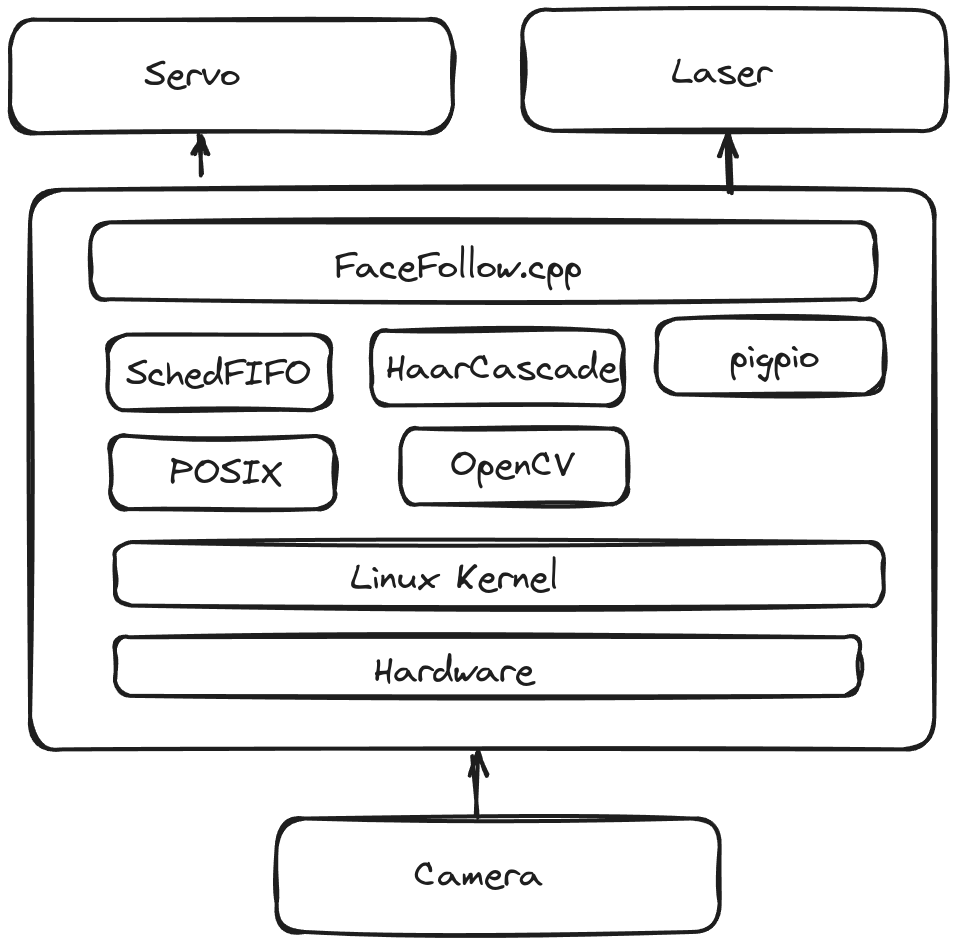
\includegraphics[scale=0.27]{figures/proof_of_concept.png}
    \caption{Different Views for Servo movement}
\end{figure}

\begin{figure}[H]
    \centering
    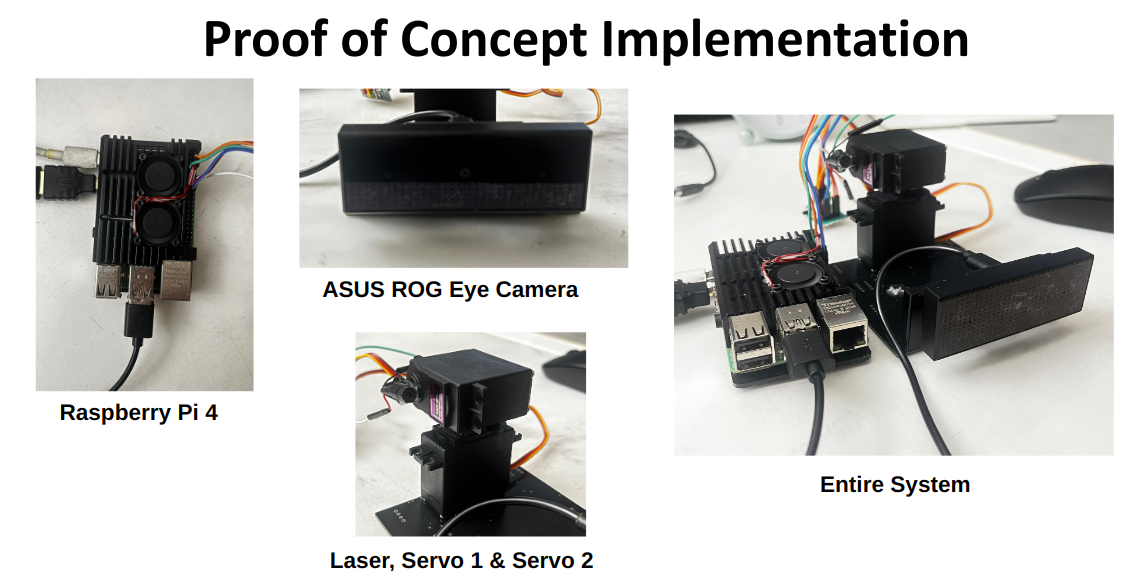
\includegraphics[scale=0.4]{figures/pf_implementation.png}
    \caption{Proof of Concept Implementation}
\end{figure}

The image represents the software architecture and components involved in the proof-of-concept implementation of the Hawkeye project. Let me explain each part in detail:
\begin{enumerate}
    \item Platform and RTOS/scheduler used
    FaceFollow.cpp: This is the main application or executable that brings together all the components and libraries required for face detection, servo control, and laser pointing.
    \item SchedFIFO: This component is responsible for scheduling the tasks or processes involved in the system. It likely implements a scheduling policy such as FIFO (First-In-First-Out) or a real-time scheduling algorithm to ensure deterministic execution and meet the real-time requirements of the system.
    HaarCascade: This is a component that uses the Haar Cascade algorithm, which is a machine learning-based approach for object detection. In this case, it is used for face detection within the captured frames.
    \item  pigpio: This is a library or component that provides hardware-timed GPIO (General-Purpose Input/Output) functionality for controlling devices like servos or motors. It is likely used in this project to control the pan and tilt servos for aiming the laser pointer.
    \item POSIX: This refers to the POSIX (Portable Operating System Interface) standard, which defines a set of APIs and libraries for developing portable and operating system-independent software. The project likely utilizes POSIX APIs for inter-process communication (IPC), threading, and other system-level operations.
    \item OpenCV: OpenCV (Open Source Computer Vision Library) is a widely used library for computer vision and image processing tasks. It is employed in this project for tasks such as frame capture, image preprocessing, and potentially face detection as well.
    \item  Linux Kernel: The Linux kernel is the core component of the Linux operating system, providing low-level services and managing hardware resources. The project is built on top of the Linux kernel, which enables the use of various system calls, device drivers, and other kernel-level functionalities.
    \item Hardware: This layer represents the physical hardware components involved in the project, such as the camera module, servos, and laser pointer.
    \item Servo: This component likely encapsulates the logic for controlling the pan and tilt servos based on the detected face coordinates.
    \item Laser: This component is responsible for managing the laser pointer, turning it on or off as needed when a face is detected and the servos are positioned correctly.
    \item Camera: This represents the camera module or device used for capturing video frames, which serves as the input for face detection and tracking.
\end{enumerate}


\subsection{Hardware Architecture}
The hardware architecture of the Hawkeye system consists of several key components that work together to achieve the desired functionality. Figure \ref{fig:hardware_arch} illustrates the high-level hardware architecture of the system.

\begin{figure}[H]
    \centering
    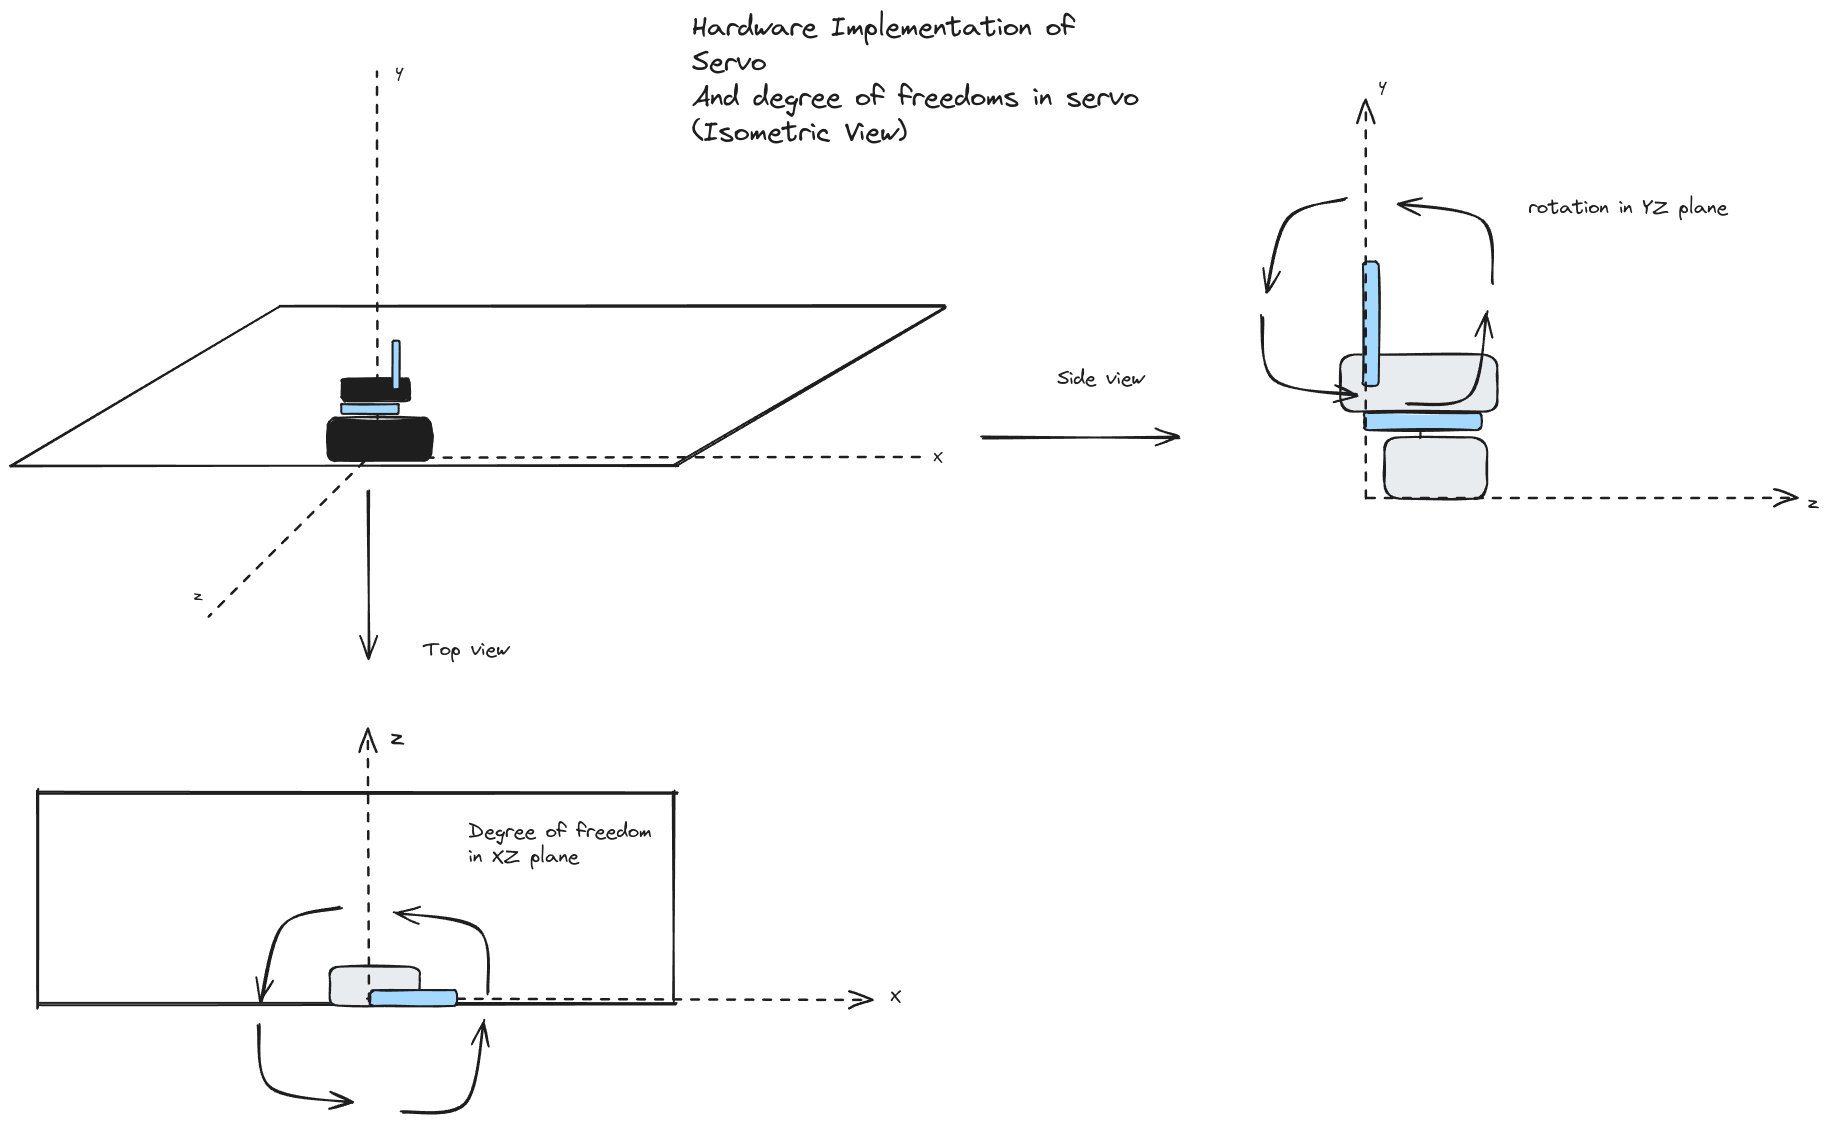
\includegraphics[scale=0.27]{figures/isometric.png}
    \caption{Different Views for Servo movement}
\end{figure}

\begin{figure}[H]
    \centering
    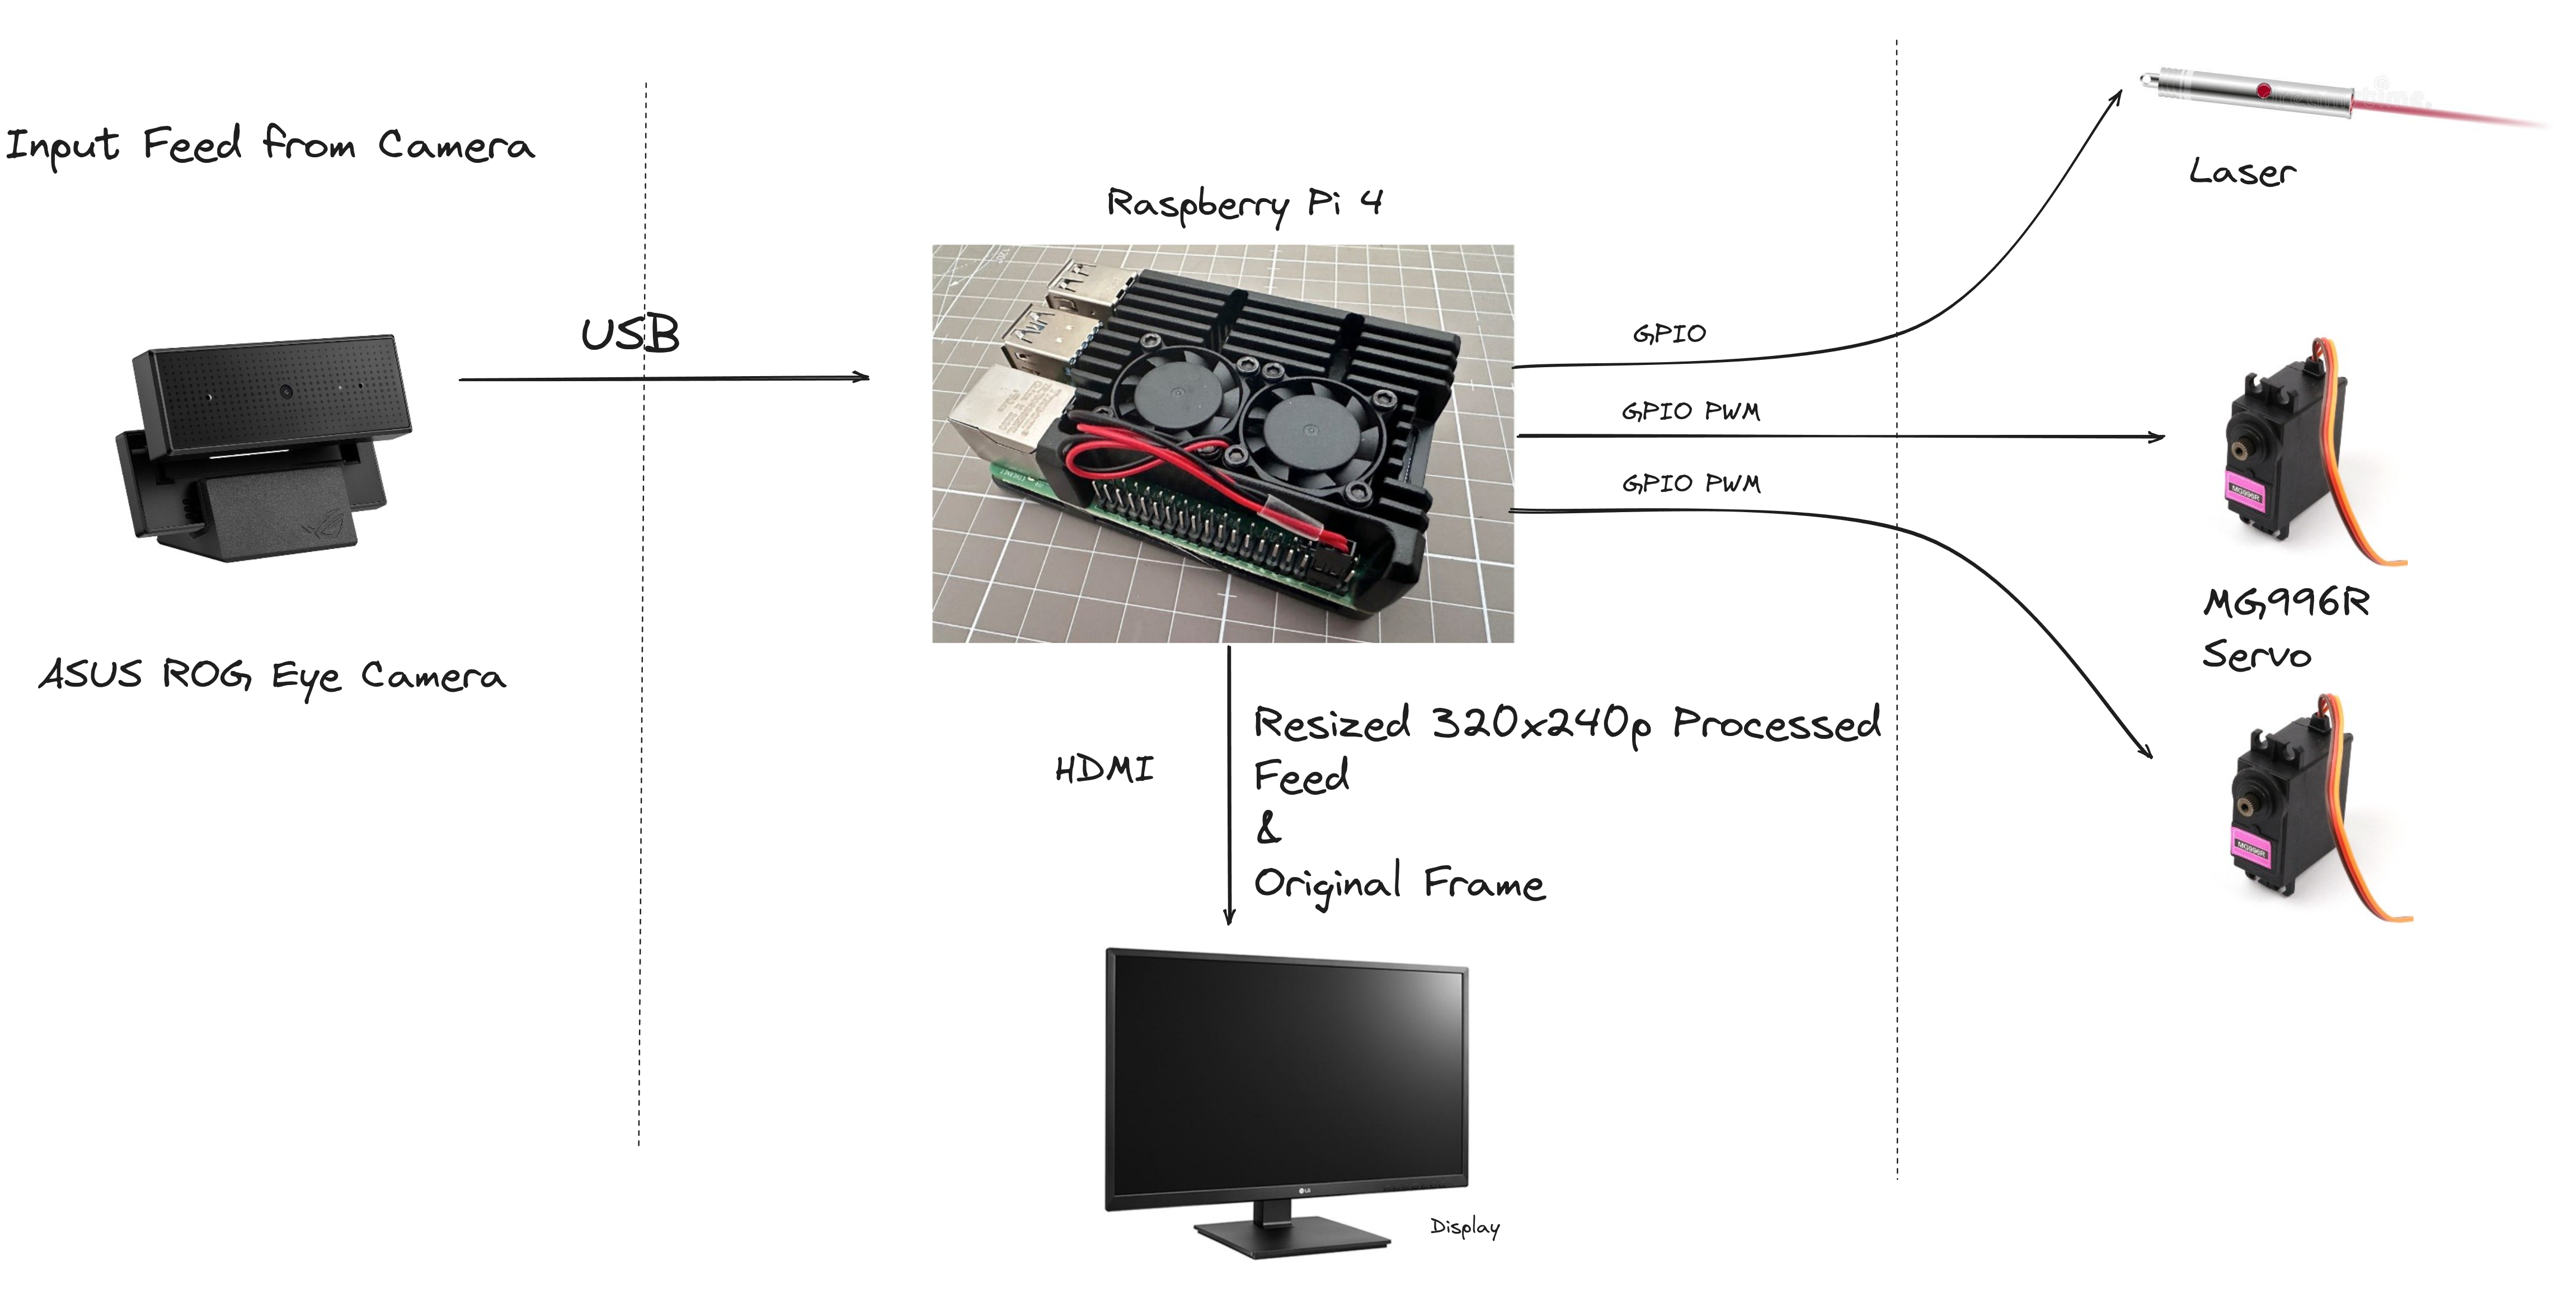
\includegraphics[scale=0.1]{figures/hw_overview.png}
    \caption{Hardware overview}
\end{figure}


The main components of the hardware architecture are:
\begin{itemize}
    \item \textbf{Raspberry PI}: we have used RPI instead of jetson nano because Raspberry PI was supporting more than one hardware pwm pins while jetson nano just supports 1 hardware pwm and we wnated to reduce the reposne time so we did not chose to do software pwm

    \item \textbf{Camera Module}: A high-quality camera module is used to capture video frames for face detection. The camera module is connected to the Jetson Nano via the MIPI CSI-2 interface, which provides a high-bandwidth and low-latency connection for image data transfer. And we have used ROG Eye Camera which is 1080p camera with 60frames throughput



    \item \textbf{Pan and Tilt Servos}: Two servos are employed to control the pan and tilt motion of the laser pointer. The pan servo is responsible for horizontal movement (left and right), while the tilt servo handles vertical movement (up and down). The servos are controlled by the PI through PWM signals.


    \item \textbf{Laser Pointer}: A laser pointer is mounted on the pan and tilt mechanism, allowing it to be aimed at the detected face. The laser pointer is controlled by the PI through a GPIO pin, which enables turning the laser on and off as needed.


\end{itemize}

\subsection{Software Architecture}
The software architecture of the Hawkeye system is designed to be modular, scalable, and efficient. It consists of several key components that work together to perform face detection, servo control, and laser pointing. Figure presents a high-level view of the software architecture.

\begin{figure}[H]
    \centering
    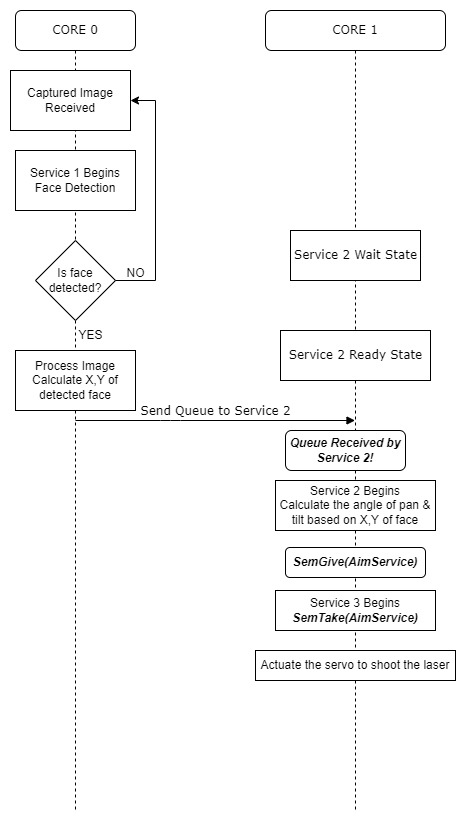
\includegraphics[scale=0.6]{figures/dfd_cfd.jpeg}
    \caption{Flow Chart}
\end{figure}



\begin{figure}[H]
    \centering
    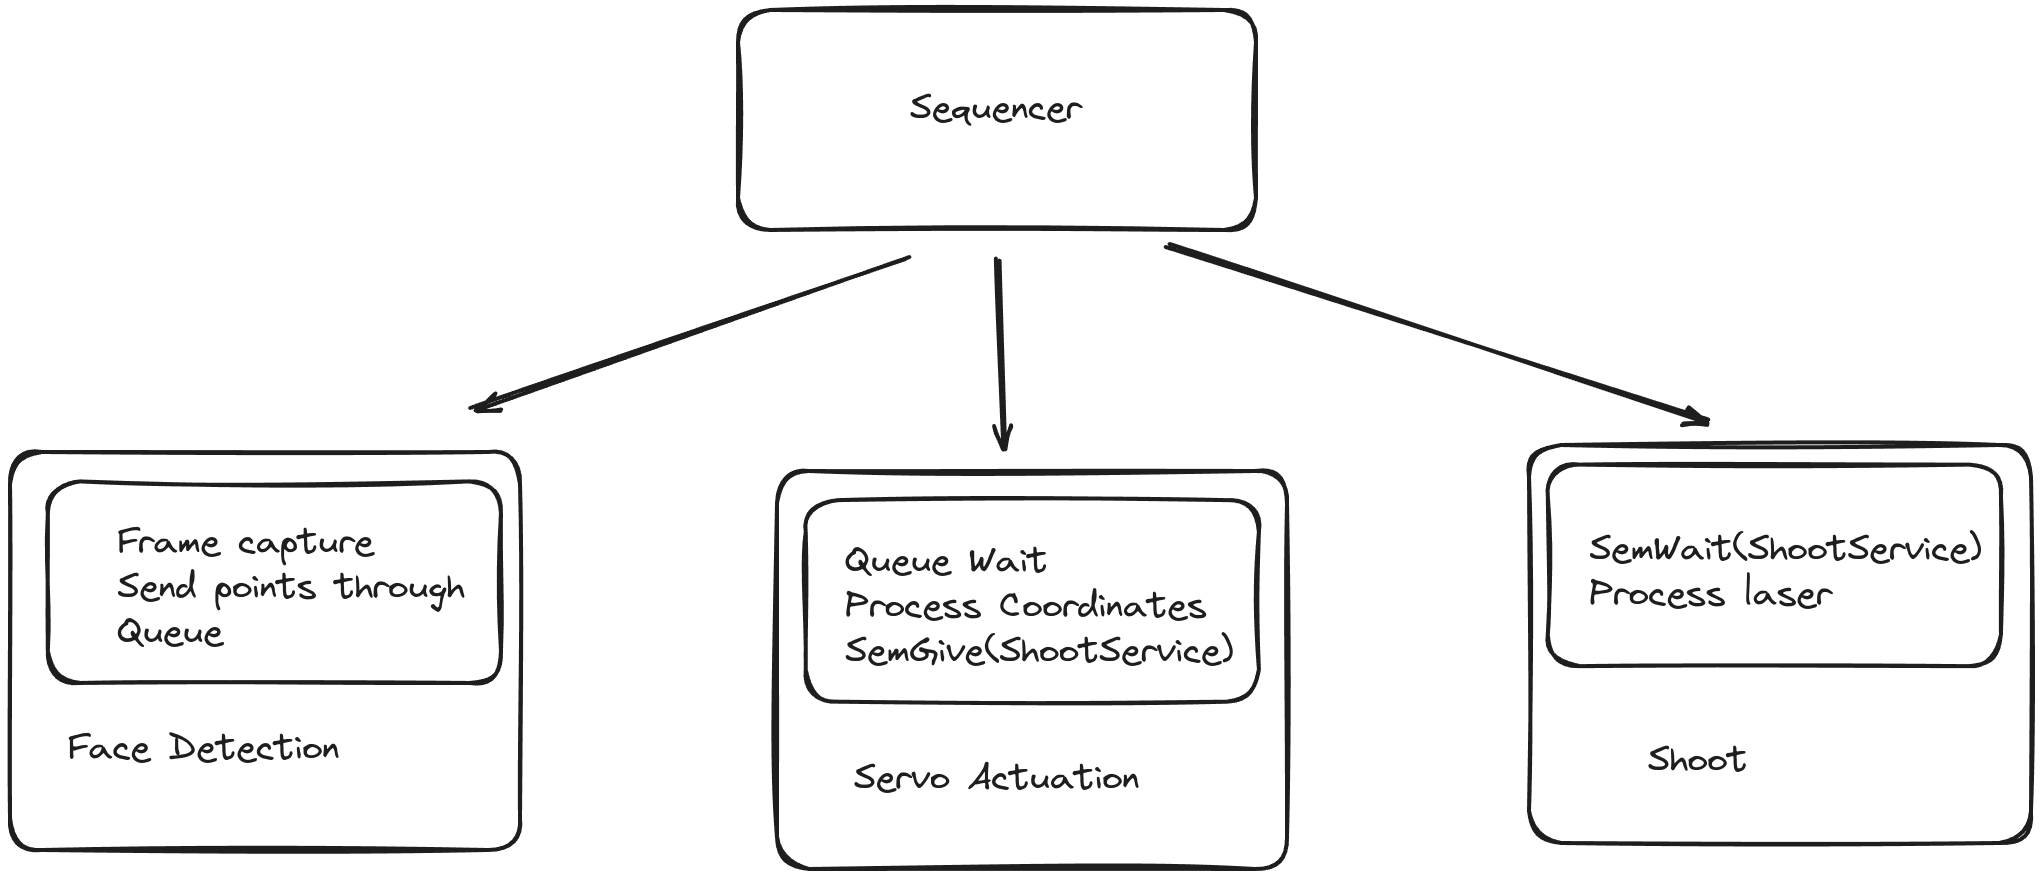
\includegraphics[scale=0.25]{figures/sw_block_diagram.png}
    \caption{Software hardware diagram}
\end{figure}


The main components of the software architecture are:
\begin{itemize}
    \item \textbf{schedular}: This is responsible for scheduling all the services with defined time period of 50 ms for each, the schedular is designed to run every 50ms and release all the semaphore at once as all the services has same period

    \item \textbf{Image Capture Module}: This module is responsible for capturing video frames from the camera module. It interfaces with the camera driver and acquires images at the desired resolution and frame rate. The captured frames are passed to the face detection module for further processing.


    \item \textbf{Face Detection Module}: The face detection module receives the captured frames from the image capture module and applies the Haar Cascade classifier to detect faces in real-time. It utilizes the OpenCV library, we are using lbp cascasde which is very high efficient algorithm for embedded system and to make execution much faster we are using 340x240 Px of resolution and we are processing grey scale image for better efficiency on low response time
          \begin{figure}[H]
              \centering
              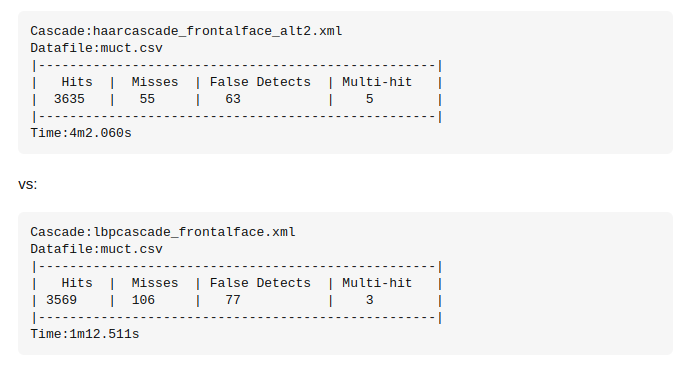
\includegraphics[scale=0.6]{figures/haarcascade.png}
              \caption{haarCascade vs lbpCascade}
          \end{figure}


    \item \textbf{Servo Control Module}: The servo control module receives the face coordinates from the face detection module and calculates the necessary pan and tilt angles to aim the laser pointer at the detected face. It uses inverse kinematics calculations to determine the required servo positions. The servo control module generates PWM signals to control the pan and tilt servos accordingly. we are using pigpio module to control the servo positioning with hardware pwm

          servo uses 20 ms of pulse width for making acutation
          \begin{figure}[H]
              \centering
              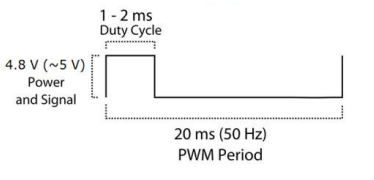
\includegraphics[scale=0.6]{figures/pwm.png}
              \caption{Servo Pulse width}
          \end{figure}

    \item \textbf{Laser Control Module}: The laser control module is responsible for turning the laser pointer on and off based on the presence of a detected face. It receives information from the face detection module and sends control signals to the laser pointer through a GPIO pin. It uses simple GPIO on off to turn on and off the module



    \item \textbf{Inter-Process Communication (IPC)}: The software modules communicate with each other using Inter-Process Communication (IPC) mechanisms. Message queues are used to pass face coordinates and other face points information between the face detection and servo actuation. Semaphores are employed to synchronize the execution of critical sections and ensure data consistency. we are sending points to the IPC queue



\end{itemize}

\subsection{Inverse kinematics}

\begin{figure}[H]
    \centering
    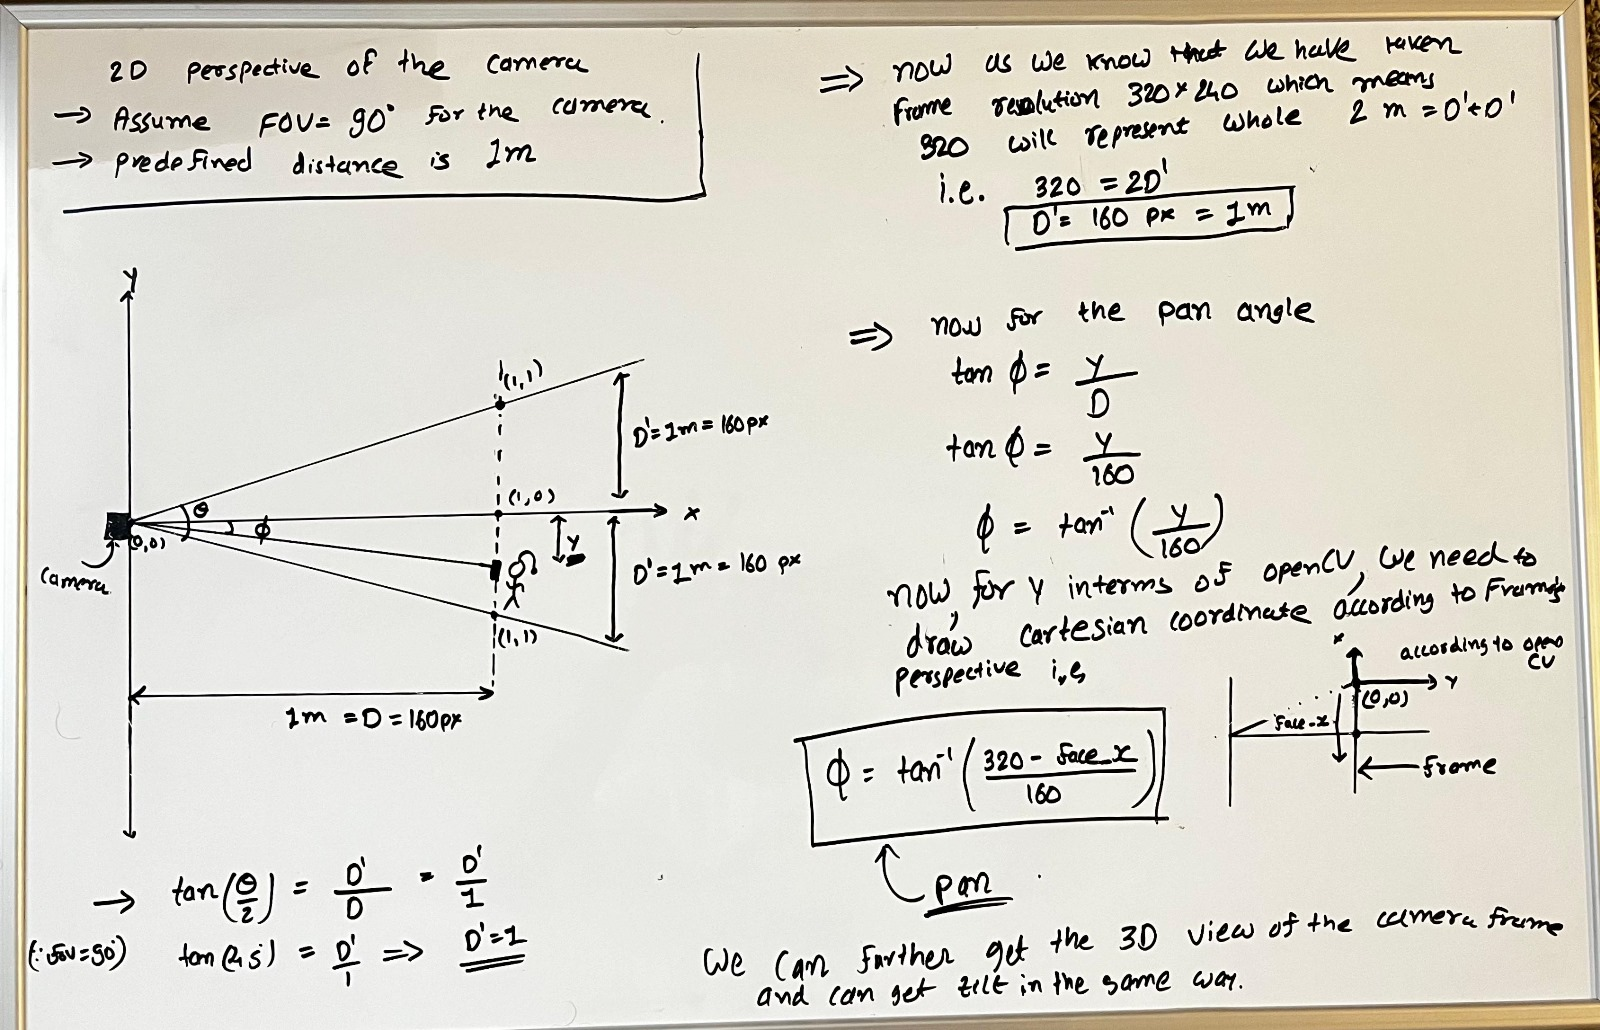
\includegraphics[scale=0.4]{figures/math.jpeg}
    \caption{Maths}
\end{figure}

In the image, we can see a 2D perspective of the camera setup. The assumptions and calculations are as follows:
\begin{enumerate}
    \item The camera's field of view (FOV) is assumed to be 90$^\circ$ for simplicity.
    \item The predefined distance between the camera and the target is 1m.
    \item The frame resolution is set to 320x240, which means that the whole frame represents a 2m = 0'-0" width at a distance of 1m.
    \item To calculate the pan angle ($\phi$), the following equation is used:
          Copy code$$\tan\phi = \frac{y}{D}$$

          Where:
          \begin{itemize}
              \item $y$ is the pixel coordinate of the target in the frame
              \item $D$ is the distance from the camera to the target (1m)
          \end{itemize}

          Substituting $D = 1m = 160px$, we get:

          $$\phi = \tan^{-1}\left(\frac{y}{160}\right)$$

    \item For the tilt angle ($\theta$), the calculation is based on the OpenCV coordinate system and the perspective projection:

          $$\theta = \tan^{-1}\left(\frac{320 - \text{face\_x}}{160}\right)$$

          Where:
          \begin{itemize}
              \item $\text{face\_x}$ is the x-coordinate of the target face in the frame
          \end{itemize}

    \item The 3D view of the camera frame can be obtained, and the tilt angle can be calculated in a similar way.

    \item The fundamental equations for converting angles to distances and vice versa are:

          $$\tan(\theta) = \frac{d'}{d}$$
          $$\tan(2.5') = \frac{d'}{1} \implies d' = 1$$

          Here, $d'$ is the distance from the camera to the target, and $d$ is the known distance of 1m.
\end{enumerate}
By using these equations and the predefined assumptions, the inverse kinematics calculations can be performed to determine the necessary pan and tilt angles for the servos to point the laser at the detected face.




\subsection{Testing and Validation}
To ensure the Hawkeye system meets its design goals and requirements, a comprehensive testing and validation plan is established. The testing and validation process covers various aspects of the system, including:

\begin{figure}[H]
    \centering
    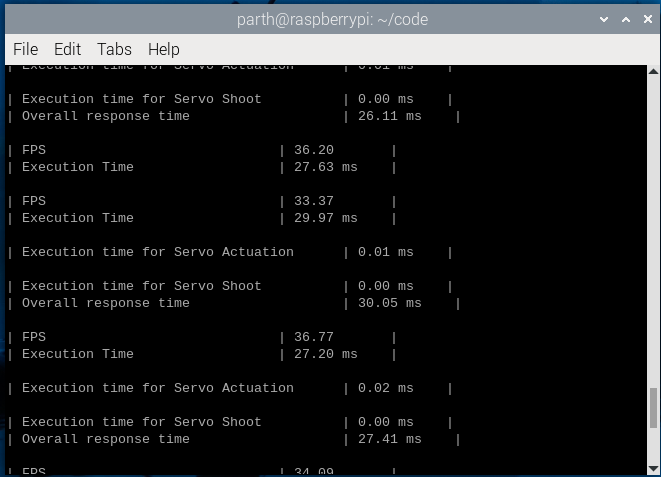
\includegraphics[scale=0.60]{figures/response_time_log.png}
    \caption{Response time from face detection}
\end{figure}

How I calculated the response time is, I calculated the response time by time-stamping the start of the face detection process and taking the difference between that and the timestamp when the servo shoot service actuated. This approach provides the overall response time, although it does not consider the input camera latency.

\begin{figure}[H]
    \centering
    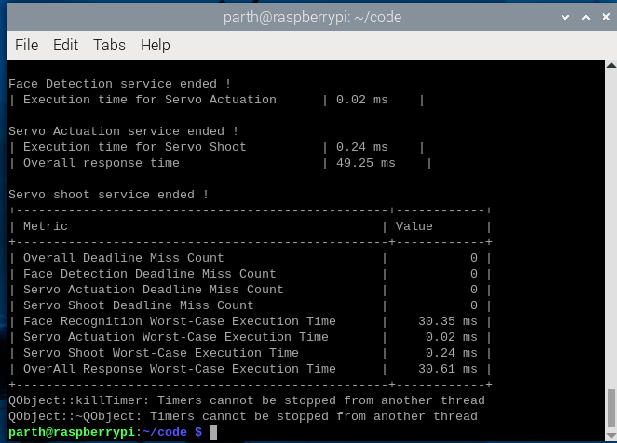
\includegraphics[scale=0.6]{figures/final_output.png}
    \caption{Final output}
\end{figure}
The final output shows that there were no deadlines missed, and the response time for the overall service set is significantly lower than the proposed deadline of 152ms, which is a positive outcome.

\begin{figure}[H]
    \centering
    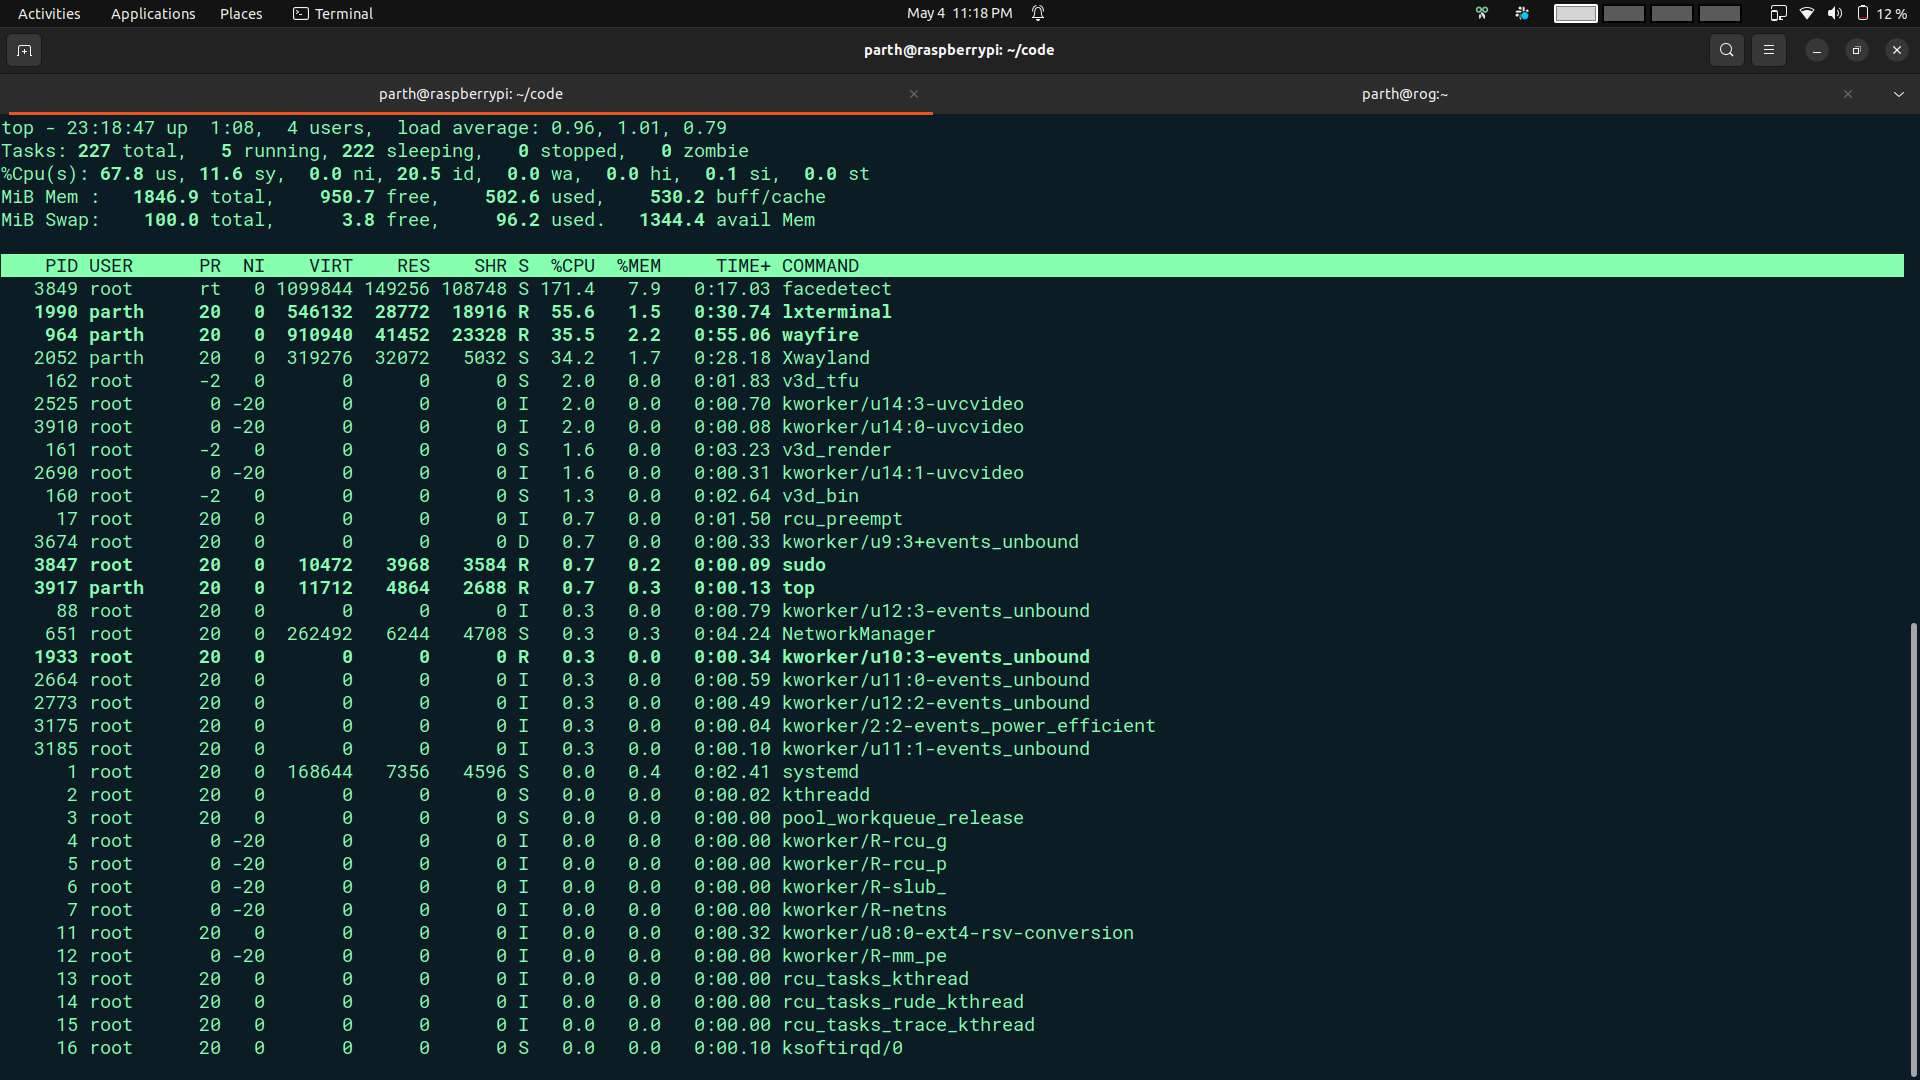
\includegraphics[scale=0.26]{figures/top.png}
    \caption{CPU Utilization}
\end{figure}

The CPU utilization data reveals that the facedetect service is consuming a significant portion of the available CPU resources. This is expected since face detection is a computationally intensive task, and the system is designed to prioritize this service for real-time performance.

\begin{enumerate}
    \item Execution Times:\\
    Servo Actuation: Executes in approximately 0.01 to 0.02 ms.\\
    Servo Shoot: Executes in 0.00 ms.\\
    Overall Response Time: Varies from 26.11 ms to 30.05 ms.\\
    Frames Per Second (FPS) and Execution Time: FPS ranges from 33.37 to 36.77.\\
    Corresponding Execution Times range from 27.20 ms to 29.97 ms.\\
    
    \item Metrics and Results from System Testing:\\
    Overall Deadline Miss Count: 0 — This indicates that all tasks were completed within their respective deadlines.
    
    \item Worst-Case Execution Time (WCET) for Key Components:\\
    Face Recognition: 29.71 ms\\
    Servo Actuation: 0.06 ms\\
    Servo Shoot: 0.01 ms\\
    Overall Response: 29.75 ms
    
    \item Analysis of Predictability and Request Frequency:
    \begin{itemize}
        \item  Predictability:
        The predictability of a real-time system is primarily assessed by its ability to consistently meet deadlines and maintain a stable worst-case execution time (WCET). In your results, the overall deadline miss count is zero, which strongly indicates that the system is highly predictable.\\
        The WCET for each component remains consistent across different test runs, which supports the reliability and predictability of the system under varying conditions.
        \item Constancy of Request Frequency:
        The FPS values show minor variations (33.37 to 36.77), suggesting a mostly stable but slightly variable request frequency. The variation in FPS might be due to the processing load or other system activities impacting the frame generation rate.
        The execution time related to these FPS values indicates that while there might be variability in how frames are processed, the system handles these variations without missing deadlines.
    \end{itemize}
   
\end{enumerate}

\section{Real-Time Analysis and Design}
The system consists of three tasks with the following parameters:

\begin{table}[H]
    \centering
    \begin{tabular}{|l|c|c|c|c|c|}
    \hline
    Task & Proposed ($C_i$) & Deadline ($D_i$) & Period ($T_i$) & Obtained $C_{avg}$ & Obtained $C_{wcet}$  \\
    \hline
    Task 1 (T1) & 35ms & 52ms & 50ms & 25ms & 26.75ms\\
    Task 2 (T2) & 4ms & 50ms & 50ms & 0.2ms & 0.24ms\\
    Task 3 (T3) & 3ms & 50ms & 50ms & 0.1ms & 0.2ms\\
    \hline
    \end{tabular}
\caption{Task Parameters}
\label{tab:task_params}
\end{table}



The obtained values from the implementation are as follows:
\begin{itemize}
\item Average Computation Times (Avg $C_i$):
\begin{itemize}
\item $C_1$ = 25ms
\item $C_2$ = 0.2ms
\item $C_3$ = 0.1ms
\end{itemize}
\item Worst Case Execution Time (WCET):
\begin{itemize}
\item $C_1$ = 26.75ms
\item $C_2$ = 0.24ms
\item $C_3$ = 0.2ms
\end{itemize}
\end{itemize}
The total deadline for all tasks is given as 152ms, which is the sum of $D_1$, $D_2$, and $D_3$ (52ms + 50ms + 50ms).
\subsection{Safety Margin Estimation}
\begin{enumerate}
\item Estimated vs Obtained Computation Time ($C_i$):
\begin{itemize}
\item Task 1:
\begin{itemize}
\item Proposed $C_1$: 35ms
\item Obtained Avg $C_1$: 25ms
\item Obtained WCET $C_1$: 26.75ms
\end{itemize}
Safety Margin: The proposed computation time has a margin since the obtained WCET (26.75ms) is lower than the proposed (35ms). The system performs better than expected by 8.25ms.
\item Task 2:
\begin{itemize}
\item Proposed $C_2$: 4ms
\item Obtained Avg $C_2$: 0.2ms
\item Obtained WCET $C_2$: 0.24ms
\end{itemize}
Safety Margin: Significant margin as the WCET is substantially lower than the proposed time, suggesting that the system has a lot of leeway (3.76ms).
\item Task 3:
\begin{itemize}
\item Proposed $C_3$: 3ms
\item Obtained Avg $C_3$: 0.1ms
\item Obtained WCET $C_3$: 0.2ms
\end{itemize}
Safety Margin: Similar to Task 2, there's a significant margin of 2.8ms, indicating much better performance than anticipated.
\end{itemize}
\item System Deadline vs Task Execution: The system's total deadline is 152ms, and the sum of the worst-case execution times for all tasks is 27.19ms (26.75ms + 0.24ms + 0.2ms). This indicates that the tasks are well within the deadline, providing a substantial safety margin in terms of time, which ensures that the system can handle additional load or delays in other processes.
\end{enumerate}
The obtained computation times being significantly lower than the proposed values indicate efficient task execution and robust system design. The system is well within safety limits, suggesting potential capacity for more tasks or higher complexity without breaching the total deadline. This analysis supports both system reliability and the potential for scalability.


\section{Future Enhancements and Scalability}
The Hawkeye system design is not only focused on meeting the current requirements but also considers future enhancements and scalability. Some potential areas for future expansion and improvement include:
\begin{itemize}
    \item \textbf{Multiple Face Tracking}: Extending the system's capabilities to track and point the laser at multiple faces simultaneously, enabling more advanced interactive applications.
          Copy code\item \textbf{Facial Recognition}: Integrating facial recognition algorithms to identify and track specific individuals, opening up possibilities for personalized interactions and security applications.

    \item \textbf{Gesture Recognition}: Incorporating gesture recognition capabilities to allow users to control the system using hand gestures or other predefined movements.

    \item \textbf{Wireless Connectivity}: Adding wireless connectivity options, such as Bluetooth or Wi-Fi, to enable remote control and integration with other devices or systems.

    \item \textbf{Miniaturization}: Exploring options for miniaturizing the hardware components and optimizing the system design for portable or wearable applications.
\end{itemize}

The system design is developed with modularity, extensibility, and scalability in mind. The software architecture is structured to allow for easy integration of new features and algorithms without significant modifications to the existing codebase. The hardware components are selected considering potential future requirements and the ability to upgrade or replace them as needed.






\section{Conclusion}

\begin{enumerate}
    \item Project Hawkeye has successfully demonstrated the integration of face recognition with precise servo actuation on a Raspberry Pi 4 without missing any deadlines.
    \item The system efficiently detects faces and actuates servos for targeted movements in real-time with an overall response time of 26.75ms.
    \item Seamless integration of the camera and servo motors was crucial. Challenges in synchronization provided insights into the complexities of real-time hardware control.
    \item Developing software to handle asynchronous tasks like image processing, software exit and servo control was key to ensuring system stability.
\end{enumerate}


\vfill
\hrule
\vspace{0.5cm}
\pagebreak
\begin{appendices}
    \section{C Code for the Implementation}
    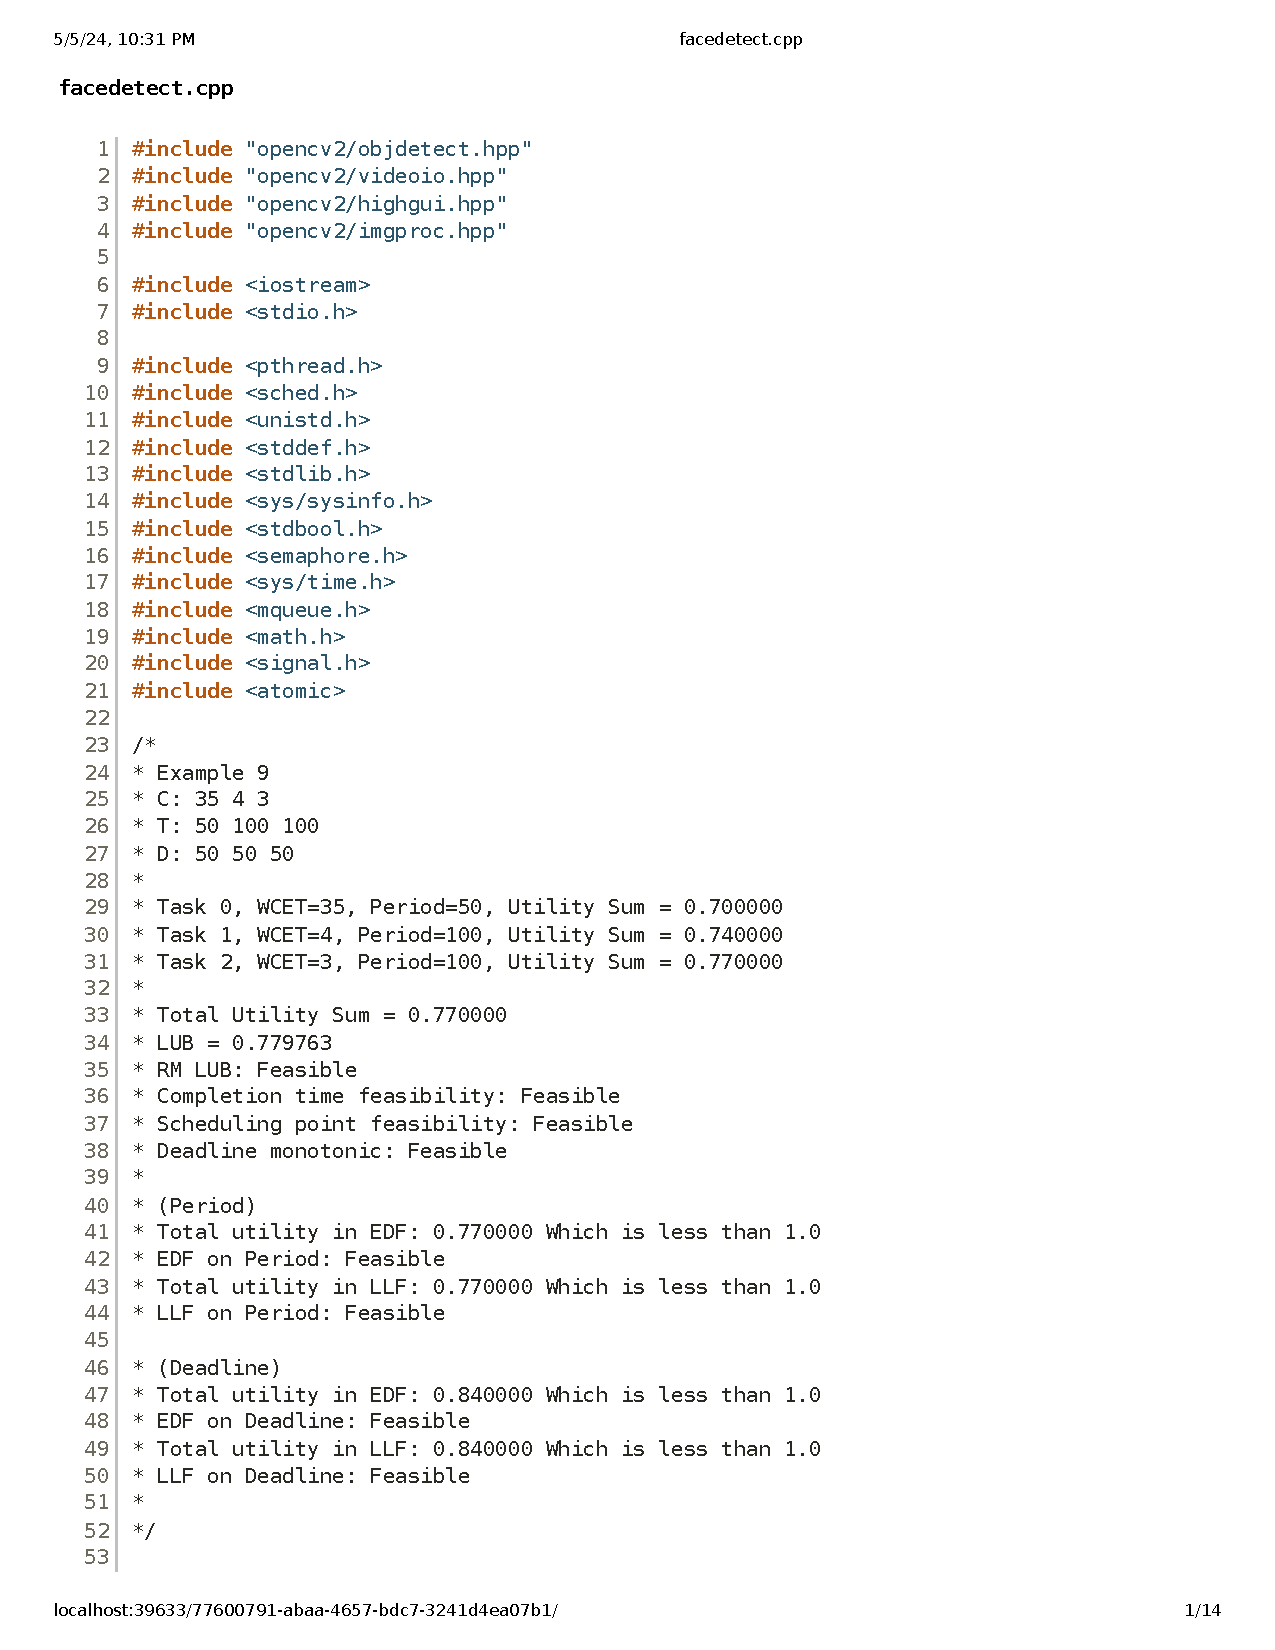
\includepdf[pages=-]{code/facedetect.cpp.pdf}
    \pagebreak
\end{appendices}


\vspace{1cm}
\hrule
\vspace{0.5cm}


%---------------------------------------------------------------------------
\end{document}
-
